%╔════════════════════════════╗
%║	  Szablon dostosował	  ║
%║	mgr inż. Dawid Kotlarski  ║
%║		  06.10.2024		  ║
%╚════════════════════════════╝
\documentclass[12pt,twoside,a4paper,openany]{article}

    % ------------------------------------------------------------------------
% PAKIETY
% ------------------------------------------------------------------------
\usepackage{tikz}
\usepackage{./tikz-uml/tikz-uml}
\usepackage{float}

%różne pakiety matematyczne, warto przejrzeć dokumentację, muszą być powyżej ustawień językowych.
\usepackage{mathrsfs}   %Różne symbole matematyczne opisane w katalogu ~\doc\latex\comprehensive. Zamienia \mathcal{L} ze zwykłego L na L-transformatę.
\usepackage{eucal}      %Różne symbole matematyczne.
\usepackage{amssymb}    %Różne symbole matematyczne.
\usepackage{amsmath}    %Dodatkowe funkcje matematyczne, np. polecenie \dfac{}{} skladajace ulamek w trybie wystawionym (porównaj $\dfrac{1}{2}$, a $\frac{1}{2}$).

%język polski i klawiatura
\usepackage[polish]{babel}
%\usepackage{qtimes} % czcionka Times new Roman
\usepackage[OT4]{polski}
%\usepackage[cp1250]{inputenc}                       %Strona kodowa polskich znaków.

%obsługa pdf'a
\usepackage[pdftex,usenames,dvipsnames]{color}      %Obsługa kolorów. Opcje usenames i dvipsnames wprowadzają dodatkowe nazwy kolorow.
\usepackage[pdftex,pagebackref=false,draft=false,pdfpagelabels=false,colorlinks=true,urlcolor=blue,linkcolor=black,citecolor=green,pdfstartview=FitH,pdfstartpage=1,pdfpagemode=UseOutlines,bookmarks=true,bookmarksopen=true,bookmarksopenlevel=2,bookmarksnumbered=true,pdfauthor={Dawid Kotlarski},pdftitle={Dokumentacja Projektowa},pdfsubject={},pdfkeywords={transient recovery voltage trv},unicode=true]{hyperref}   %Opcja pagebackref=true dotyczy bibliografii: pokazuje w spisie literatury numery stron, na których odwołano się do danej pozycji.

%bibliografia
%\usepackage[numbers,sort&compress]{natbib}  %Porządkuje zawartość odnośników do literatury, np. [2-4,6]. Musi być pod pdf'em, a styl bibliogfafii musi mieć nazwę z dodatkiem 'nat', np. \bibliographystyle{unsrtnat} (w kolejności cytowania).
\usepackage[
	backend=biber,
	style=numeric,
	sorting=none
]{biblatex}
\addbibresource{bibliografia.bib}
\usepackage{hypernat}                       %Potrzebna pakietowi natbib do wspolpracy z pakietem hyperref (wazna kolejnosc: 1. hyperref, 2. natbib, 3. hypernat).

%grafika i geometria strony
\usepackage{extsizes}           %Dostepne inne rozmiary czcionek, np. 14 w poleceniu: \documentclass[14pt]{article}.
\usepackage[final]{graphicx}
\usepackage[a4paper,left=3.5cm,right=2.5cm,top=2.5cm,bottom=2.5cm]{geometry}

%strona tytułowa
\usepackage{strona_tytulowa}

%inne
\usepackage[hide]{todo}                     %Wprowadza polecenie \todo{treść}. Opcje pakietu: hide/show. Polecenie \todos ma byc na koncu dokumentu, wszystkie \todo{} po \todos sa ignorowane.
\usepackage[basic,physics]{circ}            %Wprowadza środowisko circuit do rysowania obwodów elektrycznych. Musi byc poniżej pakietow językowych.
\usepackage[sf,bf,outermarks]{titlesec}     %Troszczy się o wygląd tytułów rozdziałów (section, subsection, ...). sf oznacza czcionkę sans serif (typu arial), bf -- bold. U mnie: oddzielna linia dla naglowku paragraph. Patrz tez: tocloft -- lepiej robi format spisu tresci.
\usepackage{tocloft}                        %Troszczy się o format spisu trsci.
\usepackage{expdlist}    %Zmienia definicję środowiska description, daje większe możliwości wpływu na wygląd listy.
\usepackage{flafter}     %Wprowadza parametr [tb] do polecenia \suppressfloats[t] (polecenie to powoduje nie umieszczanie rysunkow, tabel itp. na stronach, na ktorych jest to polecenie (np. moze byc to stroma z tytulem rozdzialu, ktory chcemy zeby byl u samej gory, a nie np. pod rysunkiem)).
\usepackage{array}       %Ładniej drukuje tabelki (np. daje wiecej miejsca w komorkach -- nie są tak ścieśnione, jak bez tego pakietu).
\usepackage{listings}    %Listingi programow.
\usepackage[format=hang,labelsep=period,labelfont={bf,small},textfont=small]{caption}   %Formatuje podpisy pod rysunkami i tabelami. Parametr 'hang' powoduje wcięcie kolejnych linii podpisu na szerokosc nazwy podpisu, np. 'Rysunek 1.'.
\usepackage{appendix}    %Troszczy się o załączniki.
\usepackage{floatflt}    %Troszczy się o oblewanie rysunkow tekstem.
\usepackage{here}        %Wprowadza dodtkowy parametr umiejscowienia rysunków, tabel, itp.: H (duże). Umiejscawia obiekty ruchome dokladnie tam gdzie są w kodzie źródłowym dokumentu.
\usepackage{makeidx}     %Troszczy się o indeks (skorowidz).

%nieużywane, ale potencjalnie przydatne
\usepackage{sectsty}           %Formatuje nagłówki, np. żeby były kolorowe -- polecenie: \allsectionsfont{\color{Blue}}.
%\usepackage{version}           %Wersje dokumentu.

% 
\usepackage{csquotes}

%============
\usepackage{longtable}			%tabelka
%============

%============
% Ustawienia listingów do kodu
%============

\usepackage{listings}
\usepackage{xcolor}

\definecolor{codegreen}{rgb}{0,0.6,0}
\definecolor{codegray}{rgb}{0.5,0.5,0.5}
\definecolor{codepurple}{rgb}{0.58,0,0.82}
\definecolor{backcolour}{rgb}{0.95,0.95,0.92}

% Definicja stylu "mystyle"
\lstdefinestyle{mystyle}{
	backgroundcolor=\color{backcolour},
	commentstyle=\color{codegreen},
	keywordstyle=\color{blue},	%magenta
	numberstyle=\tiny\color{codegray},
	stringstyle=\color{codepurple},
	basicstyle=\ttfamily\footnotesize,
	breakatwhitespace=false,
	breaklines=true,
	captionpos=b,
	keepspaces=true,
	numbers=left,
	numbersep=5pt,
	showspaces=false,
	showstringspaces=false,
	showtabs=false,
	tabsize=2
}

\lstset{style=mystyle} % Deklaracja aktywnego stylu
%===========

%PAGINA GÓRNA I DOLNA
\usepackage{fancyhdr}          %Dodaje naglowki jakie się chce.
\pagestyle{fancy}
\fancyhf{}
% numery stron w paginie dolnej na srodku
\fancyfoot[C]{\scriptsize DOKUMENTACJA PROJEKTU – PROGRAMOWANIE URZĄDZEŃ MOBILNCH \\
	\normalsize\sffamily  \thepage}


%\fancyhead[L]{\small\sffamily \nouppercase{\leftmark}}
\fancyhead[C]{\footnotesize \textit{AKADEMIA NAUK STOSOWANYCH W NOWYM SĄCZU}\\}

\renewcommand{\headrulewidth}{0.4pt}
\renewcommand{\footrulewidth}{0.4pt}

    % ------------------------------------------------------------------------
% USTAWIENIA
% ------------------------------------------------------------------------ 

% ------------------------------------------------------------------------
%   Kropki po numerach sekcji, podsekcji, itd.
%   Np. 1.2. Tytuł podrozdziału
% ------------------------------------------------------------------------
\makeatletter
    \def\numberline#1{\hb@xt@\@tempdima{#1.\hfil}}                      %kropki w spisie treści
    \renewcommand*\@seccntformat[1]{\csname the#1\endcsname.\enspace}   %kropki w treści dokumentu
\makeatother

% ------------------------------------------------------------------------
%   Numeracja równań, rysunków i tabel
%   Np.: (1.2), gdzie:
%   1 - numer sekcji, 2 - numer równania, rysunku, tabeli
%   Uwaga ogólna: o otoczeniu figure ma być najpierw \caption{}, potem \label{}, inaczej odnośnik nie działa!
% ------------------------------------------------------------------------
\makeatletter
    \@addtoreset{equation}{section} %resetuje licznik po rozpoczęciu nowej sekcji
    \renewcommand{\theequation}{{\thesection}.\@arabic\c@equation} %dodaje kropki

    \@addtoreset{figure}{section}
    \renewcommand{\thefigure}{{\thesection}.\@arabic\c@figure}

    \@addtoreset{table}{section}
    \renewcommand{\thetable}{{\thesection}.\@arabic\c@table}
\makeatother

% ------------------------------------------------------------------------
% Tablica
% ------------------------------------------------------------------------
\newenvironment{tabela}[3]
{
    \begin{table}[!htb]
    \centering
    \caption[#1]{#2}
    \vskip 9pt
    #3
}{
    \end{table}
}

% ------------------------------------------------------------------------
% Dostosowanie wyglądu pozycji listy \todos, np. zamiast 'p.' jest 'str.'
% ------------------------------------------------------------------------
\renewcommand{\todoitem}[2]{%
    \item \label{todo:\thetodo}%
    \ifx#1\todomark%
        \else\textbf{#1 }%
    \fi%
    (str.~\pageref{todopage:\thetodo})\ #2}
\renewcommand{\todoname}{Do zrobienia\ldots}
\renewcommand{\todomark}{~uzupełnić}

% ------------------------------------------------------------------------
% Definicje
% ------------------------------------------------------------------------
\def\nonumsection#1{%
    \section*{#1}%
    \addcontentsline{toc}{section}{#1}%
    }
\def\nonumsubsection#1{%
    \subsection*{#1}%
    \addcontentsline{toc}{subsection}{#1}%
    }
\reversemarginpar %umieszcza notki po lewej stronie, czyli tam gdzie jest więcej miejsca
\def\notka#1{%
    \marginpar{\footnotesize{#1}}%
    }
\def\mathcal#1{%
    \mathscr{#1}%
    }
\newcommand{\atp}{ATP/EMTP} % Inaczej: \def\atp{ATP/EMTP}

% ------------------------------------------------------------------------
% Inne
% ------------------------------------------------------------------------
\frenchspacing                      
\hyphenation{ATP/-EMTP}             %dzielenie wyrazu w danym miejscu
\setlength{\parskip}{3pt}           %odstęp pomiędzy akapitami
\linespread{1.3}                    %odstęp pomiędzy liniami (interlinia)
\setcounter{tocdepth}{4}            %uwzględnianie w spisie treści czterech poziomów sekcji
\setcounter{secnumdepth}{4}         %numerowanie do czwartego poziomu sekcji 
\titleformat{\paragraph}[hang]      %wygląd nagłówków
{\normalfont\sffamily\bfseries}{\theparagraph}{1em}{}



    %polecenia zdefiniowane w pakiecie strona_tytulowa.sty
    \title{Wirtualny Dziekanat}		%...Wpisać nazwę projektu...
    % \author{}
    \authorI{Marcin Dudek}
    \authorII{Mateusz Basiaga}		%jeśli są dwie osoby w projekcie to zostawiamy:    \authorII{}
		
	\uczelnia{AKADEMIA NAUK STOSOWANYCH \\W NOWYM SĄCZU}
    \instytut{Wydział Nauk Inżynieryjnych}
    \kierunek{Katedra Informatyki}
    \praca{DOKUMENTACJA PROJEKTOWA}
    \przedmiot{PROGRAMOWANIE URZĄDZEŃ MOBILNYCH}
    \prowadzacy{mgr inż. Dawid Kotlarski}
    \rok{2025}

%definicja składni mikrotik
\usepackage{fancyvrb}
\DefineVerbatimEnvironment{MT}{Verbatim}%
{commandchars=\+\[\],fontsize=\small,formatcom=\color{red},frame=lines,baselinestretch=1,} 
\let\mt\verb
%zakonczenie definicji składni mikrotik

\usepackage{fancyhdr}    %biblioteka do nagłówka i stopki
\begin{document}

\renewcommand{\figurename}{Rys.}    %musi byc pod \begin{document}, bo w~tym miejscu pakiet 'babel' narzuca swoje ustawienia
\renewcommand{\tablename}{Tab.}     %j.w.
\thispagestyle{empty}               %na tej stronie: brak numeru
\stronatytulowa                     %strona tytułowa tworzona przez pakiet strona_tytulowa.tex

\pagestyle{fancy}
\newpage

%formatowanie spisu treści i~nagłówków
\renewcommand{\cftbeforesecskip}{8pt}
\renewcommand{\cftsecafterpnum}{\vskip 8pt}
\renewcommand{\cftparskip}{3pt}
\renewcommand{\cfttoctitlefont}{\Large\bfseries\sffamily}
\renewcommand{\cftsecfont}{\bfseries\sffamily}
\renewcommand{\cftsubsecfont}{\sffamily}
\renewcommand{\cftsubsubsecfont}{\sffamily}
\renewcommand{\cftparafont}{\sffamily}
%koniec formatowania spisu treści i nagłówków

\tableofcontents    %spis treści
\thispagestyle{fancy}
\newpage


\newpage

%%%%%%%%%%%%%%%%%%% treść główna dokumentu %%%%%%%%%%%%%%%%%%%%%%%%%

\newpage
\section{Ogólne określenie wymagań}		%1
%Ogólne określenie wymagań i zakresu programu (Czyli zleceniodawca określa wymagania programu) 

\subsection{Główne funkcje aplikacji}

\begin{itemize}
	\item \textbf{Logowanie i autoryzacja:}
	      \\Użytkownicy powinni móc logować się za pomocą uczelnianego adresu e-mail oraz hasła. Po piewrszym logowaniu użytkownik dostanie opcje logowania za się pomocą odcisku palaca albo skanu twarzy. Możliwość logowania tyczy się zarówno dla studentów, jak i pracowników (np. wykładowcy, administracja).
	\item \textbf{Podgląd ocen i zaliczeń:}
	      \\Studenci powinni mieć możliwość przeglądania swoich ocen z egzaminów, kolokwiów oraz innych zaliczeń. Możliwość filtrowania wyników na podstawie przedmiotu, semestru czy wykładowcy.
	\item \textbf{Plan zajęć:}
	      \\Podgląd bieżącego planu zajęć z opcją aktualizacji na żywo (jeśli np. zajęcia zostaną odwołane czy przeniesione).
	\item \textbf{Harmonogram egzaminów i sesji:}
	      \\Informacje o nadchodzących egzaminach, sesjach poprawkowych i innych ważnych wydarzeniach związanych z uczelnią. Możliwość zapisywania się na egzaminy, jeżeli to wymagane.
	\item \textbf{Powiadomienia:}
	      \\Push notifications o nowych ocenach, nadchodzących zajęciach, zmianach w harmonogramie lub ważnych ogłoszeniach.
	\item \textbf{Informacje ogólne:}
	      \\Tablica ogłoszeń z najważniejszymi informacjami od uczelni, np. nowe zarządzenia rektora, wydarzenia na kampusie itp.
	\item \textbf{Profile użytkowników:}
	      \\Każdy użytkownik powinien mieć profil z podstawowymi danymi (imię, nazwisko, nr indeksu, rocznik, itd.). Możliwość aktualizacji niektórych danych kontaktowych.

	      \newpage

	\item \textbf{Responsywność i UX:}
	      \\Chcemy, żeby aplikacja była prosta i szybka w obsłudze.
	\item \textbf{Bezpieczeństwo danych: }
	      \\Chcemy, żeby dane były dobrze chronione, bo będą tu przechowywane prywatne informacje studentów. Może jakieś szyfrowanie?
	\item \textbf{Offline mode: }
	      \\Dobrze by było, gdyby część funkcji działała offline (np. podgląd planu zajęć lub ocen).
\end{itemize}

\newpage
\section{Określenie wymagań szczegółowych}		%2
%Dokładne określenie wymagań aplikacji (cel, zakres, dane wejściowe) – np. opisać przyciski, czujniki, wygląd layautu, wyświetlenie okienek. Opisać zachowanie aplikacji – co po kliknięciu, zdarzenia automatyczne. Opisać możliwość dalszego rozwoju oprogramowania. Opisać zachowania aplikacji w niepożądanych sytuacjach.

\subsection{Cel aplikacji}
Celem aplikacji jest ułatwienie studentom oraz pracownikom uczelni dostępu do kluczowych funkcji administracyjnych i informacyjnych związanych z edukacją. Aplikacja ma zastąpić tradycyjne interakcje z dziekanatem, umożliwiając szybki dostęp do ocen, planu zajęć, harmonogramu egzaminów, czy otrzymywania powiadomień.

\begin{itemize}
      \item \textbf{Zakres aplikacji:}
            \\\textbf{Studenci}: dostęp do ocen, planu zajęć, harmonogramu egzaminów, powiadomień.
            \\\textbf{Administracja: }zarządzanie danymi, kontakt ze studentami.
      \item \textbf{Platformy:}
            \\\textbf{Systemy operacyjne:} \\Android, \\iOS.
      \item \textbf{Dane wejściowe: (Logowanie użytkowników)}
            \\\textbf{Dane studentów}: nr indeksu, rocznik, oceny, plan zajęć, egzaminów, zgłoszenia do dziekanatu.
            \\\textbf{Zdarzenia dziekanatu}: zmiany w planie, ogłoszenia, nowe dokumenty, powiadomienia o ocenach.
      \item \textbf{Opis interfejsu użytkownika i elementów interaktywnych:}
            \newpage
            \textbf{Ekran logowania:  Rys. \ref{rys:ekranlogowania} (s. \pageref{rys:ekranlogowania})}
            \begin{figure}[htb!]
                  \centering
                  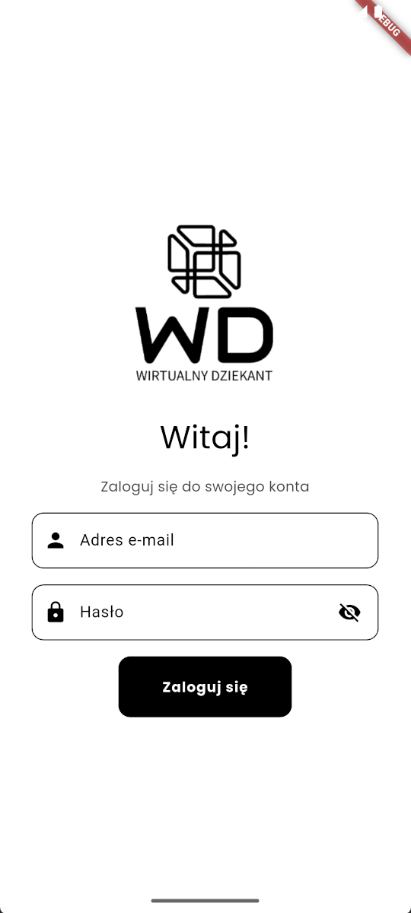
\includegraphics[width=0.65\linewidth]{rys/ekranlogowania.png}
                  \caption{Ekran logowania}
                  \label{rys:ekranlogowania}
            \end{figure}
            \newpage
            \textbf{Pola tekstowe:} „Email” oraz „Hasło”.
            \\\textbf{Przyciski:} „Zaloguj” – po kliknięciu, autoryzacja danych w tle i przejście do ekranu głównego. W przypadku błędnych danych, komunikat „Niepoprawne dane logowania”. „Zapomniałem hasła” – przekierowanie do formularza resetowania hasła.
      \item  \textbf{Ekran główny (Dashboard): Rys. \ref{rys:ekranglowny} (s. \pageref{rys:ekranglowny})}
            \begin{figure}[htb!]
                  \centering
                  
\includegraphics[width=0.8\linewidth]{rys/ekranglowny.png}
                  \caption{Ekran główny}
                  \label{rys:ekranglowny}
            \end{figure}
            \\Wyświetlane informacje: skrót do ocen, nadchodzących zajęć, powiadomienia o ważnych wydarzeniach.
            \\\textbf{Przyciski:}
            \\\textbf{„Przedmioty”} – po kliknięciu, przejście do ekranu z listą ocen, harmonogramu egzaminów z możliwością filtrowania według przedmiotu.
            \\\textbf{„Plan zajęć”} – po kliknięciu, podgląd planu zajęć (interaktywny kalendarz).
            \\\textbf{„Ustawienia”} – po kliknięciu, przejście do ustawień naszego profilu
            \\\textbf{Automatyczne zdarzenia}: wyświetlanie powiadomień push o nadchodzących zajęciach, ocenach, ważnych wydarzeniach.
            \newpage
      \item \textbf{Ekran ocen:  Rys. \ref{rys:ekranocen} (s. \pageref{rys:ekranocen})}
            \begin{figure}[htb!]
                  \centering
                  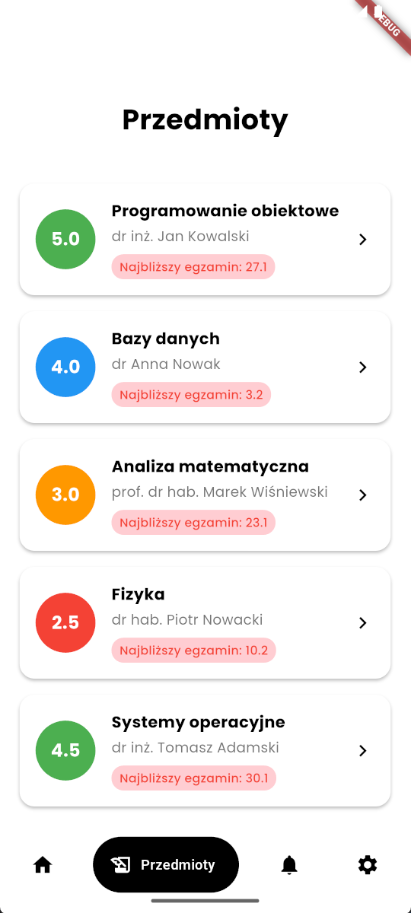
\includegraphics[width=0.65\linewidth]{rys/ekranocen.png}
                  \caption{Ekran ocen}
                  \label{rys:ekranocen}
            \end{figure}
            \newpage
            \textbf{Tabela ocen:} kolumny „Przedmiot”, „Ocena”, „Komentarz wykładowcy”, „Data”.
            \\\textbf{Opcje sortowania}: sortowanie ocen po przedmiocie, dacie.
            \\\textbf{Zachowanie:} po kliknięciu w przedmiot, otwarcie szczegółów przedmiotu (np. opis, prowadzący, historia ocen).
            Plan zajęć:

      \item \textbf{Widok kalendarza}: wyświetlanie zajęć na dany tydzień/dzień.
            \\\textbf{Funkcje interaktywne Rys. \ref{rys:ekranplanzajec} (s. \pageref{rys:ekranplanzajec})}:
            \begin{figure}[htb!]
                  \centering
                  
\includegraphics[width=0.55\linewidth]{rys/ekranplanzajec.png}
                  \caption{Ekran Planu zajęć}
                  \label{rys:ekranplanzajec}
            \end{figure}
            \newpage
            Zmiana tygodnia za pomocą przesuwania palcem (swipe left/right).
            \\Kliknięcie na zajęcia otwiera szczegóły, np. nazwisko wykładowcy, sala, godziny.
            \\Powiadomienia push: automatyczne przypomnienia o nadchodzących zajęciach z możliwością wyłączenia.

      \item \textbf{Harmonogram egzaminów Rys. \ref{rys:ekranegzaminow} (s. \pageref{rys:ekranegzaminow})}:
            \begin{figure}[htb!]
                  \centering
                  
\includegraphics[width=0.55\linewidth]{rys/ekranegzaminow.png}
                  \caption{Ekran Egzaminów}
                  \label{rys:ekranegzaminow}
            \end{figure}
            \newpage
            \textbf{Lista egzaminów}: możliwość filtrowania według przedmiotu, prowadzącego, daty.
            \\\textbf{Powiadomienia push}: przypomnienia o zbliżających się egzaminach.
            Komunikacja z dziekanatem:

      \item \textbf{Zdarzenia automatyczne}:
            \\Aplikacja będzie automatycznie wysyłać powiadomienia push o zmianach w planie zajęć, wynikach egzaminów, nowo dodanych dokumentach i ogłoszeniach.
            \\Automatyczne aktualizacje planu zajęć oraz harmonogramu egzaminów po synchronizacji z serwerem (np. co 30 minut).
      \item \textbf{Działanie offline}:
            \\Gdy brak połączenia z internetem, użytkownik ma dostęp do zapisanych wcześniej danych (plan zajęć, oceny).
      \item \textbf{Zachowanie aplikacji w niepożądanych sytuacjach}:
            \\\textbf{Brak połączenia z internetem:}
            \\Aplikacja wyświetla komunikat „Brak połączenia. Sprawdź połączenie z internetem” przy próbie wykonania operacji wymagającej synchronizacji z serwerem (np. wysłanie wiadomości do dziekanatu).
            W trybie offline: dostęp do zapisanych danych, brak możliwości interakcji z funkcjami wymagającymi połączenia.
            \\\textbf{Błędne dane logowania}:
            \\Komunikat „Niepoprawny email lub hasło” oraz możliwość ponownego wpisania danych. Pole tekstowe zostaje podświetlone na czerwono.
            \\\textbf{Serwer niedostępny}:
            \\Wyświetlenie komunikatu „Serwer dziekanatu jest obecnie niedostępny. Spróbuj ponownie później”.
            \\\textbf{Niepoprawne działanie aplikacji}:
            \\W przypadku błędu technicznego aplikacja wyświetli komunikat „Wystąpił błąd. Spróbuj ponownie” i zapisze logi błędów do późniejszej analizy przez programistów.
\end{itemize}

\newpage
\section{Projektowanie}
%Opis przygotowania narzędzi (git, visual studio). Wybór i opis bibliotek, klas. Szkic layoutów. Pseudo kody. Opisy wykorzystanych algorytmów (np. algorytm sortowania). Dokładniejsze określenie założeń i działania aplikacji, (np.: ten przycisk otworzy takie okno a w tym oknie wpisujemy takie dane).
\subsection{Przygotowanie narzędzi}

W ramach przygotowania środowiska do implementacji aplikacji wirtualnego dziekanatu oraz zarządzania wersjami kodu, wybrano zestaw narzędzi wspierających proces tworzenia oraz zapewniających automatyzację wielu czynności. W poniższych punktach opisano każde z wykorzystanych narzędzi wraz z ich rolą oraz załączonym linkiem do dokumentacji.

\begin{itemize}
	\item \textbf{Git} – system kontroli wersji, umożliwiający śledzenie zmian w kodzie oraz współpracę w zespole. Dokumentacja narzędzia: \url{https://git-scm.com/doc}\cite{www14}
	\item \textbf{VSCode} – edytor kodu źródłowego, który zapewnia wsparcie dla wielu języków programowania i umożliwia instalację rozszerzeń wspierających programowanie. Dokumentacja narzędzia: \url{https://code.visualstudio.com/docs}\cite{www3}
	\item \textbf{Android Studio} – środowisko programistyczne wykorzystywane głównie do testowania aplikacji na emulatorze Android oraz zarządzania SDK. Dokumentacja: \url{https://developer.android.com/studio/intro}\cite{www15}
	\item \textbf{Flutter SDK} – zestaw narzędzi do tworzenia aplikacji wieloplatformowych. Dokumentacja: \url{https://flutter.dev/docs}\cite{www1}
	\item \textbf{Doxygen} – narzędzie do generowania dokumentacji automatycznej na podstawie komentarzy w kodzie źródłowym. Dokumentacja narzędzia: \url{https://www.doxygen.nl/}\cite{www16}
	\item \textbf{Doxygen Awesome} – motyw graficzny dostosowujący wygląd strony wygenerowanej przez Doxygen do współczesnych standardów. Więcej informacji: \url{https://github.com/jothepro/doxygen-awesome-css}\cite{www17}
	\item \textbf{Lefthook} – narzędzie do zarządzania hookami Git, które wspiera automatyczne formatowanie, walidację kodu oraz zgodność wiadomości commitów z konwencją. Dokumentacja: \url{https://github.com/evilmartians/lefthook}\cite{www18}
	\item \textbf{Commitlint} – narzędzie do sprawdzania zgodności wiadomości commitów z konwencją \textit{Conventional Commits}. Dokumentacja: \url{https://commitlint.js.org/}\cite{www19}
	\item \textbf{GitHub Actions} – platforma do automatyzacji procesów CI/CD. Umożliwia automatyczną walidację commitów, generowanie dokumentacji oraz wersjonowanie wydań. Dokumentacja: \url{https://docs.github.com/en/actions}\cite{www20}
\end{itemize}

\subsection{Architektura systemu}

Aplikacja została zbudowana w oparciu o dwa główne komponenty:

\begin{itemize}
	\item \textbf{Backend - Payload CMS} – główny system zarządzania treścią, odpowiedzialny za:
	      \begin{itemize}
		      \item Autoryzację i uwierzytelnianie użytkowników
		      \item Przechowywanie i zarządzanie danymi aplikacji
		      \item API REST do komunikacji z aplikacją mobilną
		      \item Panel administracyjny dla pracowników uczelni
	      \end{itemize}

	\item \textbf{Firebase Cloud Messaging} – wykorzystywany wyłącznie do obsługi powiadomień push:
	      \begin{itemize}
		      \item Wysyłanie powiadomień o zmianach w planie zajęć
		      \item Informowanie o nowych ogłoszeniach
		      \item Powiadomienia o nowych wiadomościach
	      \end{itemize}
\end{itemize}

System składa się z trzech głównych komponentów \textbf{Rys. 3.1}:

\begin{figure}[h]
	\centering
	\begin{tikzpicture}[node distance=5cm]
		\node[draw,rectangle] (app) {Aplikacja mobilna (Flutter)};
		\node[draw,rectangle] (cms) [below left of=app] {Payload CMS};
		\node[draw,rectangle] (fcm) [below right of=app] {Firebase Cloud Messaging};
		\draw[->] (app) -- (cms) node[midway,above,sloped] {REST API, GraphQL};
		\draw[->] (fcm) -- (app) node[midway,above,sloped] {Powiadomienia};
	\end{tikzpicture}
	\caption{Architektura systemu}
	\label{fig:architecture}
\end{figure}
\newpage

Architektura aplikacji została zaprojektowana w modelu klient-serwer z następującymi komponentami:

\begin{itemize}
	\item \textbf{Frontend (aplikacja mobilna)}:
	      \begin{itemize}
		      \item Interfejs użytkownika w Material Design
		      \item Zarządzanie stanem aplikacji (Riverpod)
		      \item Przechowywanie danych lokalnych
		      \item Obsługa trybu offline
	      \end{itemize}

	\item \textbf{Backend (Payload CMS)}:
	      \begin{itemize}
		      \item REST API
		      \item System autoryzacji
		      \item Baza danych
		      \item Panel administracyjny
		      \item GraphQL
	      \end{itemize}

	\item \textbf{Usługi zewnętrzne}:
	      \begin{itemize}
		      \item Firebase Cloud Messaging (powiadomienia push)
	      \end{itemize}
\end{itemize}

\subsection{Framework Flutter}

Flutter to otwartoźródłowy framework opracowany przez firmę Google, służący do tworzenia wieloplatformowych aplikacji za pomocą jednej bazy kodu. Jego architektura opiera się na języku Dart, co pozwala na wydajną kompilację do kodu natywnego dla systemów Android, iOS, macOS, Windows, Linux, a także do aplikacji webowych. Główne zalety Fluttera to szybki rozwój interfejsu użytkownika, możliwość tworzenia aplikacji o wysokiej wydajności oraz wsparcie dla wzorców projektowych takich jak Material Design i Cupertino.

\subsubsection{Możliwości języka Dart}
Język Dart, na którym opiera się Flutter, jest wieloparadygmatowym językiem programowania opracowanym przez Google. Wśród jego cech charakterystycznych można wymienić:
\begin{itemize}
	\item \textbf{Statyczne typowanie}: Pozwala na wykrywanie błędów już na etapie kompilacji.
	\item \textbf{Obsługa programowania obiektowego}: Dart wspiera klasy, dziedziczenie, interfejsy i mixiny, co pozwala na tworzenie złożonych struktur kodu.
	\item \textbf{Hot Reload}: Funkcja ta umożliwia szybkie wprowadzanie zmian w kodzie i ich natychmiastowe testowanie, co przyspiesza proces rozwoju aplikacji.
	\item \textbf{Wydajność}: Kod Dart jest kompilowany do kodu natywnego, co pozwala na uzyskanie wysokiej wydajności aplikacji.
	\item \textbf{Asynchroniczność}: Obsługa asynchronicznych strumieni i przyszłości (ang. Futures) umożliwia efektywną pracę z operacjami wejścia/wyjścia.
\end{itemize}

\subsubsection{Material Design}
Flutter zapewnia natywne wsparcie dla Material Design, języka projektowania stworzonego przez Google, który definiuje zasady tworzenia nowoczesnych, responsywnych i estetycznych interfejsów użytkownika. Flutter udostępnia szeroki zestaw gotowych komponentów, takich jak:\
\begin{itemize}
	\item \texttt{AppBar} - pasek aplikacji z tytułem i opcjonalnymi akcjami.
	\item \texttt{FloatingActionButton} - unoszący się przycisk akcji.
	\item \texttt{Drawer} - wysuwane menu nawigacyjne.
	\item \texttt{Card} - komponent do wyświetlania informacji w stylu kart.
	\item \texttt{TextField} - pole tekstowe do wprowadzania danych.
\end{itemize}
Dzięki temu deweloperzy mogą tworzyć spójne interfejsy użytkownika zgodne z najnowszymi trendami projektowymi.

\subsubsection{Pakiety i narzędzie Pub}
Pub to menedżer pakietów dla Fluttera i języka Dart, który umożliwia łatwe zarządzanie bibliotekami i zależnościami w projekcie. Za pomocą Pub można:
\begin{itemize}
	\item Dodawać gotowe pakiety z \texttt{pub.dev}, takich jak \texttt{http} do pracy z protokołem HTTP czy \texttt{provider} do zarządzania stanem aplikacji.
	\item Tworzyć własne pakiety i udostępniać je społeczności programistów.
	\item Aktualizować zależności i zarządzać ich wersjami, co pozwala na utrzymanie zgodności między różnymi komponentami aplikacji.
\end{itemize}

Dzięki Pub, rozwój aplikacji w Flutterze staje się bardziej efektywny, a społeczność użytkowników ma dostęp do bogatego ekosystemu bibliotek i narzędzi.

\subsection{Payload CMS}
Payload CMS to nowoczesny system zarządzania treścią (CMS), który został zaprojektowany z myślą o deweloperach. Jest to w pełni konfigurowalny headless CMS oparty na Node.js, który umożliwia łatwe tworzenie i zarządzanie treściami w aplikacjach internetowych. Payload wyróżnia się prostotą integracji, elastycznością oraz wysoką wydajnością.

\subsubsection{Funkcje i zalety Payload CMS}
Payload CMS oferuje szereg zaawansowanych funkcji, które ułatwiają pracę deweloperom:
\begin{itemize}
	\item \textbf{Headless CMS}: Payload działa jako API-first CMS, co oznacza, że treści można dostarczać do dowolnego frontendowego frameworka lub aplikacji.
	\item \textbf{Elastyczna konfiguracja}: System pozwala na definiowanie niestandardowych schematów treści (ang. schemas) przy użyciu kodu JavaScript lub TypeScript.
	\item \textbf{Bezpieczeństwo}: Payload oferuje wbudowane mechanizmy uwierzytelniania, zarządzania użytkownikami i ról, a także obsługę protokołu OAuth.
	\item \textbf{Interfejs użytkownika}: Payload udostępnia intuicyjny panel administracyjny, który jest generowany automatycznie na podstawie zdefiniowanych schematów.
	\item \textbf{API REST i GraphQL}: Payload obsługuje zarówno REST API, jak i GraphQL, co umożliwia łatwy dostęp do danych na różne sposoby.
	\item \textbf{Wtyczki i rozszerzalność}: Payload wspiera wtyczki, co pozwala na rozszerzanie jego funkcjonalności o dodatkowe moduły.
\end{itemize}

\subsubsection{Proces tworzenia projektu}
Tworzenie projektu w Payload CMS przebiega w kilku prostych krokach:
\begin{enumerate}
	\item \textbf{Instalacja}: Payload można zainstalować za pomocą menedżera pakietów npm lub yarn:
	      \textbf{Listing. \ref{lst:cms} (s. \pageref{lst:cms})}:
	      \begin{lstlisting}[language=C++, caption=Tworznie cms , label={lst:cms}]
    npx create-payload-app my-project
    \end{lstlisting}
	\item \textbf{Definicja schematów}: Deweloperzy definiują kolekcje danych w formie kodu, np.:
	      \textbf{Listing. \ref{lst:cms2} (s. \pageref{lst:cms2})}:
	      \begin{lstlisting}[language=C++, caption=Przykład deklaracji w Payload CMS, label={lst:cms2}]
    const Posts = {
      slug: 'posts',
      fields: [
        {
          name: 'title',
          type: 'text',
        },
        {
          name: 'content',
          type: 'richText',
        },
      ],
    };
    \end{lstlisting}
	\item \textbf{Uruchomienie serwera}: Po skonfigurowaniu projektu, serwer Payload można uruchomić poleceniem \texttt{npm run dev}.
	\item \textbf{Integracja z frontendem}: Payload CMS udostępnia API, które można wykorzystać w aplikacjach frontendowych, np. z wykorzystaniem React, Next.js czy Vue.js.
\end{enumerate}

\subsubsection{Przykładowe zastosowania Payload CMS}
Payload CMS znajduje zastosowanie w wielu typach projektów, takich jak:
\begin{itemize}
	\item Strony internetowe i blogi,
	\item Aplikacje mobilne i webowe wymagające dynamicznych treści,
	\item Platformy e-commerce,
	\item Systemy zarządzania użytkownikami.
\end{itemize}

Dzięki swojej elastyczności i nowoczesnemu podejściu Payload CMS stanowi doskonałe rozwiązanie dla deweloperów poszukujących prostego w użyciu, ale jednocześnie potężnego narzędzia do zarządzania treścią.

\subsection{Projekt interfejsu użytkownika aplikacji}

\subsubsection{Style i motywy}
\begin{itemize}
	\item Spójny system projektowy Material Design 3
	\item Wsparcie dla motywu jasnego i ciemnego
	\item Dynamiczne dostosowanie do różnych rozmiarów ekranów
	\item Responsywne komponenty UI
\end{itemize}

\subsubsection{Nawigacja}
\begin{itemize}
	\item Menu dolne z 4 głównymi sekcjami:
	      \begin{itemize}
		      \item Panel główny
		      \item Powiadomienia
		      \item Wiadomości
		      \item Ustawienia
	      \end{itemize}
	\item Nawigacja stosowa między ekranami
	\item Gesty nawigacyjne (swipe)
\end{itemize}

\subsection{Model danych}

\subsubsection{Główne encje}
\begin{itemize}
	\item \textbf{User}:
	      \begin{itemize}
		      \item Dane podstawowe (imię, nazwisko, email)
		      \item Rola (student/wykładowca/admin)
		      \item Ustawienia (język, powiadomienia)
	      \end{itemize}

	\item \textbf{Schedule}:
	      \begin{itemize}
		      \item Przedmiot
		      \item Data i czas
		      \item Sala
		      \item Prowadzący
	      \end{itemize}

	\item \textbf{Notification}:
	      \begin{itemize}
		      \item Typ
		      \item Treść
		      \item Data
		      \item Odbiorcy
	      \end{itemize}
\end{itemize}

\subsection{Bezpieczeństwo}

\begin{itemize}
	\item \textbf{Autoryzacja}:
	      \begin{itemize}
		      \item JWT tokens
		      \item Refresh tokens
		      \item Szyfrowanie danych wrażliwych
	      \end{itemize}

	\item \textbf{Walidacja danych}:
	      \begin{itemize}
		      \item Walidacja formularzy
		      \item Sanityzacja danych wejściowych
		      \item Obsługa błędów
	      \end{itemize}
\end{itemize}

\subsection{Synchronizacja danych}

\begin{itemize}
	\item \textbf{Cache lokalny}:
	      \begin{itemize}
		      \item Przechowywanie planu zajęć
		      \item Buforowanie ogłoszeń
		      \item Ustawienia użytkownika
	      \end{itemize}

	\item \textbf{Strategia synchronizacji}:
	      \begin{itemize}
		      \item Automatyczna synchronizacja w tle
		      \item Ręczne odświeżanie danych
		      \item Kolejkowanie operacji offline
	      \end{itemize}
\end{itemize}
\subsection{Diagram UML}
% Klasa Student
\begin{figure}[H]
	\centering
	\begin{tikzpicture}
		\umlclass[x=0, y=0]{Student}{
			- id: int \\
			- firstName: String \\
			- middleName: dynamic \\
			- familyName: String \\
			- coursesOfStudy: List<CoursesOfStudy> \\
			- dateOfBirth: DateTime \\
			- updatedAt: DateTime \\
			- createdAt: DateTime \\
			- collection: String \\
			- loginAttempts: int
		}{
			+ factory Student.fromJson(Map<String, dynamic> json) \\
			+ toJson(): Map<String, dynamic>
		}
	\end{tikzpicture}
	\caption{Klasa Student}
	\label{fig:class-student}
\end{figure}
\newpage
% Klasa Schedule
\begin{figure}[H]
	\centering
	\begin{tikzpicture}
		\umlclass[x=0, y=0]{Schedule}{
			- id: int \\
			- courseOfStudy: int \\
			- weekAfullTimeSchedule: WeekFullTimeSchedule \\
			- weekAPartTimeSchedule: WeekPartTimeSchedule \\
			- weekBfullTimeSchedule: WeekFullTimeSchedule \\
			- weekBPartTimeSchedule: WeekPartTimeSchedule \\
			- updatedAt: DateTime \\
			- createdAt: DateTime
		}{
			+ factory Schedule.fromJson(Map<String, dynamic> json) \\
			+ toJson(): Map<String, dynamic>
		}
	\end{tikzpicture}
	\caption{Klasa Schedule}
	\label{fig:class-schedule}
\end{figure}

% Klasa CoursesOfStudy
\begin{figure}[H]
	\centering
	\begin{tikzpicture}
		\umlclass[x=0, y=0]{CoursesOfStudy}{
			- id: int \\
			- fieldOfStudy: String \\
			- faculty: Faculty \\
			- schedule: Schedule \\
			- courseType: String \\
			- levelOfStudy: String \\
			- obtainedTitle: String \\
			- numberOfSemesters: int \\
			- currentSemester: int \\
			- startDate: DateTime \\
			- endDate: DateTime \\
			- updatedAt: DateTime \\
			- createdAt: DateTime
		}{
			+ factory CoursesOfStudy.fromJson(Map<String, dynamic> json) \\
			+ toJson(): Map<String, dynamic>
		}
	\end{tikzpicture}
	\caption{Klasa CoursesOfStudy}
	\label{fig:class-coursesofstudy}
\end{figure}

\subsection{Design backendu}
Modularna i skalowalna architektura backendu stanowi kluczowy element współczesnych systemów programistycznych. Projektowanie backendu oparte na najlepszych praktykach pozwala na łatwe zarządzanie, rozwijanie oraz integrację z różnorodnymi usługami. Poniżej przedstawiono kluczowe aspekty, które powinny być uwzględnione przy projektowaniu nowoczesnego backendu.

\subsubsection{Budowa modułowa}
Budowa modułowa pozwala na podzielenie systemu na niezależne komponenty, które mogą być rozwijane i utrzymywane autonomicznie. Dzięki temu:
\begin{itemize}
	\item Każdy moduł jest odpowiedzialny za określony zestaw funkcjonalności, co ułatwia ich implementację i testowanie.
	\item Możliwe jest równoległe rozwijanie różnych części systemu przez różne zespoły deweloperskie.
	\item Moduły można łatwo wymieniać lub rozszerzać bez wpływu na pozostałe części systemu.
\end{itemize}

\subsubsection{Łatwa skalowalność}
Aby backend był skalowalny, należy:
\begin{itemize}
	\item Projektować usługi zgodnie z zasadami mikroserwisów lub serverless, co pozwala na niezależne skalowanie poszczególnych funkcjonalności.
	\item Korzystać z elastycznych baz danych, takich jak NoSQL, które łatwo adaptują się do wzrostu danych.
	\item Wykorzystać load balancery do równoważenia obciążenia między serwerami.
	\item Używać narzędzi monitorujących, takich jak Prometheus czy Grafana, aby efektywnie zarządzać wydajnością systemu.
\end{itemize}

\subsubsection{Internacjonalizacja}
Internacjonalizacja (i18n) jest kluczowa dla systemów działających na rynkach globalnych. Kluczowe kroki to:
\begin{itemize}
	\item Używanie narzędzi takich jak gettext lub formatów JSON/YAML do przechowywania tłumaczeń.
	\item Projektowanie interfejsów API, które wspierają wielojęzyczność, np. poprzez parametry \texttt{locale}.
	\item Uwzględnianie lokalnych formatów dat, liczb i walut w zależności od ustawień użytkownika.
	\item Testowanie systemu pod kątem poprawności wyświetlania treści w różnych językach.
\end{itemize}

\subsubsection{Bezpieczeństwo i zarządzanie danymi}
Bezpieczeństwo danych i użytkowników to fundament każdego backendu. Zaleca się:
\begin{itemize}
	\item Stosowanie szyfrowania danych w ruchu (TLS/SSL) oraz w spoczynku.
	\item Implementację autoryzacji i uwierzytelniania z wykorzystaniem standardów takich jak OAuth 2.0 czy JWT.
	\item Regularne testy bezpieczeństwa w celu wykrywania podatności.
	\item Spełnianie wymogów prawnych, takich jak RODO (GDPR) w przypadku zarządzania danymi osobowymi.
\end{itemize}

\subsubsection{Monitorowanie i obsługa błędów}
Monitorowanie systemu pozwala na szybkie wykrywanie i rozwiązywanie problemów. Warto:
\begin{itemize}
	\item Korzystać z narzędzi takich jak Sentry do logowania błędów.
	\item Implementować mechanizmy automatycznego restartu usług w przypadku awarii.
	\item Tworzyć raporty wydajnościowe i systemy alertów w celu bieżącej kontroli stanu backendu.
\end{itemize}

Modularna budowa, łatwa skalowalność, internacjonalizacja, bezpieczeństwo oraz monitorowanie stanowią podstawę dobrze zaprojektowanego backendu, który może sprostać wymaganiom współczesnych aplikacji.

\newpage
\section{Implementacja}		%4
%Wkleić szkielet kodu, wraz z komentarzami. Opisać zmienne, struktury do czego służą. Opisać procedury, metody co wykonują. Opisać nowe zdefiniowane klasy. Opisać dziedziczenie. Opisać nowo utworzone pliki za co odpowiadają.

\subsection{Struktura projektu}

Projekt został podzielony na następujące główne katalogi:

\begin{itemize}
  \item \textbf{lib/} - główny katalog z kodem źródłowym
        \begin{itemize}
          \item \textbf{models/} - modele danych
          \item \textbf{screens/} - widoki aplikacji
          \item \textbf{utils/} - narzędzia pomocnicze
          \item \textbf{providers/} - zarządzanie stanem
          \item \textbf{services/} - warstwa komunikacji z API
          \item \textbf{widgets/} - komponenty wielokrotnego użytku
        \end{itemize}
\end{itemize}

\subsection{Modele danych}

\subsubsection{Model użytkownika \textbf{Listing. \ref{lst:user-model} (s. \pageref{lst:user-model})}}
\begin{lstlisting}[language=C++, caption=Model użytkownika, label={lst:user-model}]
class AppUser {
  final String uid;
  final String email;
  
  AppUser({
    required this.uid,
    required this.email,
  });
}
\end{lstlisting}
Model `AppUser` reprezentuje użytkownika aplikacji. Zawiera unikalny identyfikator `uid` oraz adres email `email`.
\newpage
\subsubsection{Model wydarzenia \textbf{Listing. \ref{lst:event-model} (s. \pageref{lst:event-model})}}
\begin{lstlisting}[language=C++, caption=Model wydarzenia, label={lst:event-model}]
class Event {
  final String title;
  final TimeOfDay startTime;
  final TimeOfDay endTime;
  final String room;
  final String type;
  final String lecturer;
  final DateTime date;

  Event({
    required this.title,
    required this.startTime,
    required this.endTime,
    required this.room,
    required this.lecturer,
    required this.type,
    required this.date,
  });
}
\end{lstlisting}
Model `Event` reprezentuje wydarzenie w aplikacji. Zawiera informacje takie jak tytuł `title`, czas rozpoczęcia `startTime`, czas zakończenia `endTime`, sala `room`, typ zajęć `type`, wykładowca `lecturer` oraz data `date`.

\subsection{Zarządzanie stanem}

\subsubsection{Dostawca motywu \textbf{Listing. \ref{lst:theme-provider} (s. \pageref{lst:theme-provider})}}
\begin{lstlisting}[language=C++, caption=Provider motywu, label={lst:theme-provider}]
final darkModeProvider = StateNotifierProvider<DarkModeNotifier, bool>((ref) {
  return DarkModeNotifier();
});

class DarkModeNotifier extends StateNotifier<bool> {
  DarkModeNotifier() : super(false);

  void toggleDarkMode(bool value) {
    state = value;
  }
}
\end{lstlisting}
Provider `darkModeProvider` zarządza stanem trybu ciemnego w aplikacji. Klasa `DarkModeNotifier` dziedziczy po `StateNotifier<bool>` i umożliwia przełączanie trybu ciemnego za pomocą metody `toggleDarkMode`.

\subsection{Usługi API}

\subsubsection{Serwis powiadomień \textbf{Listing. \ref{lst:notification-service} (s. \pageref{lst:notification-service})}}
\begin{lstlisting}[language=C++, caption=Serwis powiadomień, label={lst:notification-service}]
class FirebaseApi {
  final _firebaseMessaging = FirebaseMessaging.instance;

  Future<void> initNotifications() async {
    await _firebaseMessaging.requestPermission();
    final token = await _firebaseMessaging.getToken();
    print('Token: $token');
  }

  void handleMessage(RemoteMessage? message) {
    if (message == null) return;
  }
}
\end{lstlisting}
Klasa `FirebaseApi` odpowiada za obsługę powiadomień push. Metoda `initNotifications` inicjalizuje powiadomienia, a `handleMessage` obsługuje otrzymane wiadomości.

\subsection{Komponenty wielokrotnego użytku}

\subsubsection{Przycisk stylizowany \textbf{Listing. \ref{lst:styled-button} (s. \pageref{lst:styled-button})}}
\begin{lstlisting}[language=C++, caption=Komponent przycisku, label={lst:styled-button}]
class StyledButton extends StatelessWidget {
  final VoidCallback onPressed;
  final Widget child;

  const StyledButton({
    Key? key,
    required this.onPressed,
    required this.child,
  }) : super(key: key);

  @override
  Widget build(BuildContext context) {
    return ElevatedButton(
      onPressed: onPressed,
      style: ElevatedButton.styleFrom(
        shape: RoundedRectangleBorder(
          borderRadius: BorderRadius.circular(12),
        ),
      ),
      child: child,
    );
  }
}
\end{lstlisting}
Komponent `StyledButton` to stylizowany przycisk, który można wielokrotnie używać w aplikacji. Przyjmuje funkcję `onPressed` oraz widget `child` jako argumenty.

\subsection{Logika biznesowa}

\subsubsection{Filtrowanie wydarzeń \textbf{Listing. \ref{lst:event-filtering} (s. \pageref{lst:event-filtering})}}
\begin{lstlisting}[language=C++, caption=Filtrowanie wydarzeń, label={lst:event-filtering}]
List<Event> filterEvents(List<Event> events, DateTime selectedDay) {
  return events
    .where((event) => isSameDay(event.date, selectedDay))
    .toList()
    ..sort((a, b) {
      final aStart = DateTime(
        selectedDay.year, 
        selectedDay.month, 
        selectedDay.day,
        a.startTime.hour,
        a.startTime.minute
      );
      final bStart = DateTime(
        selectedDay.year,
        selectedDay.month,
        selectedDay.day,
        b.startTime.hour,
        b.startTime.minute
      );
      return aStart.compareTo(bStart);
    });
}
\end{lstlisting}
Funkcja `filterEvents` filtruje i sortuje wydarzenia na podstawie wybranego dnia `selectedDay`.

\subsection{Wygodne SDK do komunikacji z backendem}

Poniższy kod implementuje klasę \texttt{WirtualnySdk}, która pełni rolę wygodnego narzędzia do komunikacji z backendem. Dzięki wykorzystaniu wzorców projektowych takich jak \textbf{Singleton} oraz \textbf{Factory}, zapewniono efektywną inicjalizację i dostęp do komponentów SDK.

\subsubsection{Wzorzec Singleton}
Wzorzec \textbf{Singleton} umożliwia istnienie tylko jednej instancji klasy \texttt{WirtualnySdk} w całej aplikacji. Dzięki temu wszystkie moduły aplikacji mają dostęp do tej samej konfiguracji SDK i mogą współdzielić zasoby. W kodzie poniżej mechanizm Singleton realizowany jest poprzez:

\begin{itemize}
  \item Prywatne pole statyczne \texttt{\_instance}, które przechowuje instancję klasy.
  \item Prywatny konstruktor \texttt{\_internal}, który zapobiega tworzeniu instancji z zewnątrz.
  \item Publiczną metodę \texttt{initialize()}, która inicjalizuje SDK i ustawia konfigurację.
  \item Getter \texttt{instance}, który zwraca istniejącą instancję SDK lub zgłasza wyjątek, jeśli SDK nie zostało zainicjalizowane.
\end{itemize}

Kod weryfikuje, czy SDK zostało już zainicjalizowane. Próba wielokrotnej inicjalizacji prowadzi do zgłoszenia wyjątku \textbf{Listing. \ref{lst:event-sdk} (s. \pageref{lst:event-sdk})}:

\begin{lstlisting}[language=C++, caption=Zgłoszenie wyjątku,  label={lst:event-sdk}]
if (_instance != null) {
    throw Exception('WirtualnySdk has already been initialized.');
}
\end{lstlisting}

\subsubsection{Wzorzec Factory}
Wzorzec \textbf{Factory} umożliwia tworzenie instancji klasy poprzez wywołanie metody \texttt{factory}. W kodzie zastosowano fabrykę do implementacji uproszczonego dostępu do obiektu SDK \textbf{Listing. \ref{lst:event-factory} (s. \pageref{lst:event-factory})}:

\begin{lstlisting}[language=C++, caption=Wzorzec Factory,  label={lst:event-factory}]
factory WirtualnySdk() {
    return instance;
}
\end{lstlisting}

Fabryka zwraca już istniejącą instancję klasy \texttt{WirtualnySdk}, co integruje się z mechanizmem Singleton. Umożliwia to bezpieczny i wygodny dostęp do SDK bez potrzeby ręcznego zarządzania instancją.

\subsubsection{Modularna budowa SDK}
Klasa \texttt{WirtualnySdk} zapewnia dostęp do modułów \texttt{auth} oraz \texttt{notifications}, odpowiedzialnych za uwierzytelnianie i obsługę powiadomień. Każdy z modułów jest instancjonowany jako prywatne pole i dostępny za pośrednictwem getterów \textbf{Listing. \ref{lst:event-auth} (s. \pageref{lst:event-auth})}:

\begin{lstlisting}[language=C++, caption=WirtualnyAuth,  label={lst:event-auth}]
final WirtualnyAuth _auth = WirtualnyAuth();
final WirtualnyNotifications _wirtualnyNotifications =
    WirtualnyNotifications();

WirtualnyAuth get auth => _auth;
WirtualnyNotifications get notifications => _wirtualnyNotifications;
\end{lstlisting}

Dzięki takiemu podejściu aplikacja ma zapewnioną modularność i łatwość rozbudowy SDK o kolejne komponenty.

\subsubsection{Podsumowanie}
Implementacja klasy \texttt{WirtualnySdk} pokazuje skuteczne wykorzystanie wzorców Singleton i Factory, dzięki czemu SDK jest łatwe w użyciu, bezpieczne i zgodne z zasadami dobrej architektury. Klasa zapewnia wygodny dostęp do kluczowych funkcji, takich jak uwierzytelnianie i powiadomienia, co czyni ją centralnym punktem integracji z backendem.

\subsection{Wysyłanie powiadomień o ogłoszeniach - implementacja backendowa}

Poniższy kod w języku TypeScript przedstawia proces wysyłania powiadomień typu FCM (Firebase Cloud Messaging) do wielu urządzeń jednocześnie w formie powiadomień o ogłoszeniach. Obsługiwane są zarówno urządzenia Android, jak i iOS. Kod zawiera również mechanizm logowania oraz obsługi błędów. \textbf{Listing. \ref{lst:fcm_notification} (s. \pageref{lst:fcm_notification})}

\begin{lstlisting}[language=c++, caption={Implementacja wysyłania powiadomień FCM}, label={lst:fcm_notification}]
try {
  getMessaging().sendEachForMulticast({
    tokens: fcmTokens,
    notification: {
      title: doc.subject,
      body: stripHtml(doc.content_html).result,
    },
    data: {
      type: 'announcement',
      id: doc.id.toString(),
      click_action: 'FLUTTER_NOTIFICATION_CLICK',
    },
    android: {
      priority: doc.priority === 'high' ? 'high' : 'normal',
      notification: {
        clickAction: 'FLUTTER_NOTIFICATION_CLICK',
      },
    },
    apns: {
      headers: {
        'apns-priority': doc.priority === 'high' ? '10' : '5',
      },
    },
    fcmOptions: {
      analyticsLabel: 'announcement',
    },
  });

  if (enableLogs) {
    payload.logger.info(
      `Successfully sent FCM notification for '${collectionSlug}' document with ID: '${doc.id}''.`,
    );
  }
} catch (error: unknown) {
  const msg = error instanceof Error ? error.message : error;
  throw new APIError(
    `Failed to send FCM notification for '${collectionSlug}' document with ID: '${doc.id}': ${msg}'.`,
  );
}
\end{lstlisting}

\textbf{Opis działania:}
\begin{itemize}
  \item \textbf{Powiadomienia FCM:} Funkcja \texttt{sendEachForMulticast} umożliwia wysyłanie powiadomień do grupy urządzeń zdefiniowanych w tablicy \texttt{fcmTokens}.
  \item \textbf{Struktura powiadomienia:} Powiadomienia zawierają tytuł (\texttt{title}), treść (\texttt{body}) oraz dane dodatkowe (\texttt{data}), takie jak typ powiadomienia (\texttt{announcement}) czy identyfikator dokumentu (\texttt{id}).
  \item \textbf{Obsługa platform:}
        \begin{itemize}
          \item \textbf{Android:} Ustawiane są priorytety (\texttt{high} lub \texttt{normal}) oraz akcje kliknięcia.
          \item \textbf{iOS:} Nagłówki \texttt{apns-priority} definiują priorytet wiadomości.
        \end{itemize}
  \item \textbf{Logowanie:} W przypadku sukcesu wysyłania, logowana jest informacja o wysłaniu powiadomienia.
  \item \textbf{Obsługa błędów:} W przypadku błędu, rzucany jest wyjątek \texttt{APIError} z odpowiednim komunikatem.
\end{itemize}

\subsection{Integracja z backendem}

Aplikacja komunikuje się z backendem Payload CMS poprzez REST API. Główne endpointy:

\begin{itemize}
  \item \texttt{/api/auth/login} - logowanie użytkownika
  \item \texttt{/api/events} - zarządzanie planem zajęć
  \item \texttt{/api/subjects} - zarządzanie przedmiotami
  \item \texttt{/api/notifications} - zarządzanie powiadomieniami
\end{itemize}
Uwierzytelnianie odbywa się poprzez tokeny JWT przechowywane w \texttt{SharedPreferences}.

\subsection{Deployment}

Projekt PayloadCMS\cite{github-backend} został wdrożony na serwerze Ubuntu\cite{backend} z wykorzystaniem Nginx jako reverse proxy, certyfikatu SSL od Certbota, zarządzania DNS przez Cloudflare oraz narzędzi takich jak PM2 i pnpm. PayloadCMS w wersji 3 działa na frameworku Next.js, co zapewnia wydajność i elastyczność w budowie aplikacji.

\subsubsection{Uruchamianie aplikacji za pomocą pnpm i PM2}

Do zarządzania zależnościami projektu wykorzystano pnpm, co pozwala na szybsze instalacje oraz oszczędność miejsca na dysku. W katalogu projektu wszystkie niezbędne zależności zostały zainstalowane poleceniem \textbf{Listing. \ref{lst:event-pnpm} (s. \pageref{lst:event-pnpm})}:
\begin{lstlisting}[language=C++, caption=Instalacja pnpm,  label={lst:event-pnpm}]
pnpm install
\end{lstlisting}

Po zakończeniu konfiguracji i upewnieniu się, że aplikacja działa lokalnie w trybie produkcyjnym (\texttt{pnpm build} oraz \texttt{pnpm start}), PayloadCMS został uruchomiony i monitorowany za pomocą PM2. PM2 jest używany do zarządzania procesami aplikacji w tle, co zapewnia niezawodność oraz możliwość automatycznego restartu w razie awarii. Aplikację uruchomiono w trybie produkcyjnym następująco \textbf{Listing. \ref{lst:event-pnpm2} (s. \pageref{lst:event-pnpm2})}:
\begin{lstlisting}[language=C++, caption=Uruchamianie pnpm,  label={lst:event-pnpm2}]
pm2 start npm --name "payload-cms" -- start
\end{lstlisting}

PM2 zapewnia również możliwość monitorowania procesów oraz logów \textbf{Listing. \ref{lst:event-pnpm3} (s. \pageref{lst:event-pnpm3})}:
\begin{lstlisting}[language=C++, caption=Sprawdzenie status oraz logów przy pomocy pnpm,  label={lst:event-pnpm3}]
pm2 status
pm2 logs payload-cms
\end{lstlisting}

\subsubsection{Konfiguracja Nginx jako Reverse Proxy}

Nginx został skonfigurowany jako reverse proxy, aby przekierowywać ruch HTTP/HTTPS na serwer PayloadCMS działający na porcie aplikacji. Oto przykład konfiguracji wirtualnego hosta \textbf{Listing. \ref{lst:event-pnpm4} (s. \pageref{lst:event-pnpm4})}:
\begin{lstlisting}[language=C++, caption=Konfiguracja nginx,  label={lst:event-pnpm4}]
server {
    listen 80;
    server_name example.com www.example.com;

    location / {
        proxy_pass http://localhost:3000;
        proxy_http_version 1.1;
        proxy_set_header Upgrade $http_upgrade;
        proxy_set_header Connection 'upgrade';
        proxy_set_header Host $host;
        proxy_cache_bypass $http_upgrade;
    }
}
\end{lstlisting}

Po dodaniu powyższej konfiguracji Nginx został przeładowany \textbf{Listing. \ref{lst:event-pnpm5} (s. \pageref{lst:event-pnpm5})}:
\begin{lstlisting}[language=C++, caption=przeładowanie konfiguracji,  label={lst:event-pnpm5}]
sudo systemctl reload nginx
\end{lstlisting}

\subsubsection{SSL i Cloudflare}

Domenę skonfigurowano z użyciem Cloudflare oraz certyfikatu SSL wygenerowanego przez Certbota. Certbot zaktualizował konfigurację Nginx w celu obsługi HTTPS \textbf{Listing. \ref{lst:event-pnpm6} (s. \pageref{lst:event-pnpm6})}:
\begin{lstlisting}[language=C++, caption=Ustawienie cerbota,  label={lst:event-pnpm6}]
sudo certbot --nginx -d example.com -d www.example.com
\end{lstlisting}

Cloudflare zostało skonfigurowane do zarządzania DNS (rekordy \texttt{A} i \texttt{CNAME}) oraz aktywowano tryb \texttt{Full SSL/TLS encryption mode}.

\subsubsection{Podsumowanie}

Dzięki wykorzystaniu pnpm do zarządzania zależnościami oraz PM2 do nadzorowania procesu aplikacji, PayloadCMS w wersji 3 (opartej na Next.js) działa stabilnie i wydajnie. Dodatkowo Nginx, Certbot oraz Cloudflare zapewniają bezpieczeństwo, wysoką dostępność i optymalizację dla użytkowników końcowych.

\subsection{Przygotowanie pakietu .apk aplikacji mobilnej}

Proces przygotowania pakietu \texttt{.apk} dla aplikacji mobilnej stworzonej w Flutterze obejmuje kilka kroków, od konfiguracji projektu po generowanie gotowego pliku instalacyjnego. Poniżej przedstawiono szczegóły całego procesu.

\subsubsection{Konfiguracja projektu Flutter}

Przed rozpoczęciem procesu budowy upewniono się, że projekt Flutter jest odpowiednio skonfigurowany do pracy w środowisku produkcyjnym:
\begin{enumerate}
  \item Plik \texttt{pubspec.yaml} został zaktualizowany, a wszystkie zależności zostały zainstalowane \textbf{Listing. \ref{lst:event-pnpm7} (s. \pageref{lst:event-pnpm7})}:
        \begin{lstlisting}[language=C++, caption=Pobranie pakietów w flutterze,  label={lst:event-pnpm7}]
    flutter pub get
    \end{lstlisting}
  \item Zdefiniowano odpowiednią konfigurację w pliku \texttt{AndroidManifest.xml}, w tym \texttt{applicationId}, pozwolenia (\texttt{permissions}) oraz ustawienia dotyczące wersji aplikacji (\texttt{versionCode} i \texttt{versionName}).
  \item Plik \texttt{build.gradle} w module \texttt{app} zawierał właściwą konfigurację dla środowiska produkcyjnego, w tym \texttt{minSdkVersion} i \texttt{targetSdkVersion}.
\end{enumerate}

\subsubsection{Budowanie pakietu .apk}

Pakiet \texttt{.apk} został wygenerowany za pomocą polecenia Fluttera do budowy w trybie produkcyjnym \textbf{Listing. \ref{lst:event-pnpm8} (s. \pageref{lst:event-pnpm8})}:
\begin{lstlisting}[language=C++, caption=Budowa oficjalnego pakietu .apk,  label={lst:event-pnpm8}]
flutter build apk --release
\end{lstlisting}

Wygenerowany plik \texttt{app-release.apk} został zapisany w katalogu \texttt{build/app/outputs/flutter-apk/}.

\subsubsection{Podpisywanie aplikacji}

Aby aplikacja mogła być zainstalowana na urządzeniach użytkowników, wymagane było jej podpisanie:
\begin{enumerate}
  \item Wygenerowano klucz kryptograficzny (\texttt{.keystore}) za pomocą narzędzia \texttt{keytool} \textbf{Listing. \ref{lst:event-pnpm9} (s. \pageref{lst:event-pnpm9})}:
        \begin{lstlisting}[language=C++, caption=Generowanie kluczu krypotraficznego,  label={lst:event-pnpm9}]
    keytool -genkey -v -keystore my-release-key.jks \
        -keyalg RSA -keysize 2048 -validity 10000 \
        -alias my-key-alias
    \end{lstlisting}
  \item Plik \texttt{my-release-key.jks} został umieszczony w katalogu \texttt{android/app/}.
  \item W pliku \texttt{android/key.properties} zdefiniowano dane dostępowe do klucza \textbf{Listing. \ref{lst:event-pnpm10} (s. \pageref{lst:event-pnpm10})}:
        \begin{lstlisting}[language=C++, caption=Dane dostępowe do klucza,  label={lst:event-pnpm10}]
    storePassword=your-store-password
    keyPassword=your-key-password
    keyAlias=my-key-alias
    storeFile=path/to/my-release-key.jks
    \end{lstlisting}
  \item Plik \texttt{build.gradle} został zaktualizowany, aby uwzględnić konfigurację podpisu \textbf{Listing. \ref{lst:event-pnpm11} (s. \pageref{lst:event-pnpm11})}:
        \begin{lstlisting}[language=C++, caption=Uwzględnienie podpisu w pliku build.gradle,  label={lst:event-pnpm11}]
    android {
        signingConfigs {
            release {
                keyAlias 'my-key-alias'
                keyPassword 'your-key-password'
                storeFile file('path/to/my-release-key.jks')
                storePassword 'your-store-password'
            }
        }
        buildTypes {
            release {
                signingConfig signingConfigs.release
            }
        }
    }
    \end{lstlisting}
\end{enumerate}

\subsubsection{Testowanie pakietu}

Gotowy pakiet \texttt{.apk} został przetestowany na urządzeniach fizycznych i emulatorach, aby upewnić się, że działa poprawnie. Weryfikację przeprowadzono za pomocą polecenia \textbf{Listing. \ref{lst:event-pnpm12} (s. \pageref{lst:event-pnpm12})}:
\begin{lstlisting}[language=C++, caption=Testowanie pakietu,  label={lst:event-pnpm12}]
flutter install
\end{lstlisting}

\subsubsection{Podsumowanie}

Pakiet \texttt{.apk} aplikacji mobilnej został przygotowany i podpisany, co pozwala na jego dystrybucję do użytkowników poprzez ręczną instalację lub publikację w sklepie Google Play. Wykorzystanie Fluttera oraz właściwa konfiguracja środowiska produkcyjnego gwarantują wysoką wydajność oraz zgodność z różnymi urządzeniami Android.

\newpage
\section{Testowanie}	%5
%Opisujemy testy, sprawdzamy czy nie generuje błędów.

\subsection{Logowanie do aplikacji}
W tabeli nr. \ref{tab:tabelka001} (s. \pageref{tab:tabelka001}) możemy zobaczyć że logowanie przebiega pomyślnie, jeśli dane wprowadzone przez użytkownika są poprawne, w przypadku podania niepoprawnego adresu e-mailu, hasła lub błędu składowego, logowanie zostanie odrzucone.
\begin{table}[h!]
	\centering
	\begin{tabularx}{\textwidth}{|X|>{\arraybackslash}m{0.45\textwidth}|X|X|}
		\hline
		\textbf{Funkcja} & \textbf{Typ Danych}               & \textbf{Rezultat} & \textbf{Działanie} \\ \hline
		Logowanie        & Poprawne dane                     & Działa            & Poprawnie          \\ \hline
		                 & Poprawny email, błędne hasło      & Błąd              & Poprawnie          \\ \hline
		                 & Błędny email, poprawne hasło      & Błąd              & Poprawnie          \\ \hline
		                 & Błędne dane                       & Błąd              & Poprawnie          \\ \hline
		                 & Hasło, które ma mniej niż 6 liter & Błąd              & Poprawnie          \\ \hline
		                 & Błędny format adresu email        & Błąd              & Poprawnie          \\ \hline
	\end{tabularx}
	\caption{Logowanie}
	\label{tab:tabelka001}
\end{table}

\subsection{Powiadomienia push}
W tabeli nr. \ref{tab:tabelka007} (s. \pageref{tab:tabelka007}) możemy zobaczyć, że powiadomienia push są wysyłane i odbierane poprawnie.
\begin{table}[h!]
	\centering
	\begin{tabularx}{\textwidth}{|X|>{\arraybackslash}m{0.45\textwidth}|X|X|}
		\hline
		\textbf{Funkcja}   & \textbf{Typ Danych}          & \textbf{Rezultat} & \textbf{Działanie} \\ \hline
		Powiadomienia push & Poprawne dane                & Działa            & Poprawnie          \\ \hline
		                   & Brak połączenia z internetem & Błąd              & Poprawnie          \\ \hline
		                   & Błędne dane                  & Błąd              & Poprawnie          \\ \hline
	\end{tabularx}
	\caption{Powiadomienia push}
	\label{tab:tabelka007}
\end{table}
\newpage
\subsection{Biometria}
W tabeli nr. \ref{tab:tabelka008} (s. \pageref{tab:tabelka008}) możemy zobaczyć, że funkcja biometrii działa poprawnie, jeśli użytkownik udzielił odpowiednich uprawnień.
\begin{table}[h!]
	\centering
	\begin{tabularx}{\textwidth}{|X|>{\arraybackslash}m{0.45\textwidth}|X|X|}
		\hline
		\textbf{Funkcja} & \textbf{Typ Danych}      & \textbf{Rezultat} & \textbf{Działanie} \\ \hline
		Biometria        & Udzielone uprawnienia    & Działa            & Poprawnie          \\ \hline
		                 & Brak uprawnień           & Błąd              & Poprawnie          \\ \hline
		                 & Błędne dane biometryczne & Błąd              & Poprawnie          \\ \hline
	\end{tabularx}
	\caption{Biometria}
	\label{tab:tabelka008}
\end{table}

\subsection{Synchronizacja danych}
W tabeli nr. \ref{tab:tabelka009} (s. \pageref{tab:tabelka009}) możemy zobaczyć, że synchronizacja danych działa poprawnie, zarówno w trybie online, jak i offline.
\begin{table}[h!]
	\centering
	\begin{tabularx}{\textwidth}{|X|>{\arraybackslash}m{0.45\textwidth}|X|X|}
		\hline
		\textbf{Funkcja}      & \textbf{Typ Danych}          & \textbf{Rezultat}     & \textbf{Działanie} \\ \hline
		Synchronizacja danych & Połączenie z internetem      & Działa                & Poprawnie          \\ \hline
		                      & Brak połączenia z internetem & Działa (tryb offline) & Poprawnie          \\ \hline
		                      & Błędne dane                  & Błąd                  & Poprawnie          \\ \hline
	\end{tabularx}
	\caption{Synchronizacja danych}
	\label{tab:tabelka009}
\end{table}

\subsection{Autoryzacja i uprawnienia}
W tabeli nr. \ref{tab:tabelka010} (s. \pageref{tab:tabelka010}) możemy zobaczyć, że autoryzacja i zarządzanie uprawnieniami działa poprawnie.
\begin{table}[h!]
	\centering
	\begin{tabularx}{\textwidth}{|X|>{\arraybackslash}m{0.45\textwidth}|X|X|}
		\hline
		\textbf{Funkcja} & \textbf{Typ Danych} & \textbf{Rezultat} & \textbf{Działanie} \\ \hline
		Autoryzacja      & Poprawne dane       & Działa            & Poprawnie          \\ \hline
		                 & Błędne dane         & Błąd              & Poprawnie          \\ \hline
		                 & Brak uprawnień      & Błąd              & Poprawnie          \\ \hline
	\end{tabularx}
	\caption{Autoryzacja i uprawnienia}
	\label{tab:tabelka010}
\end{table}
\newpage
\subsection{Robienie zdjęcia i wysyłanie do serwera}
W tabeli nr. \ref{tab:tabelka011} (s. \pageref{tab:tabelka011}) możemy zobaczyć, że funkcja robienia zdjęcia i wysyłania go do serwera działa poprawnie.
\begin{table}[h!]
	\centering
	\begin{tabularx}{\textwidth}{|X|>{\arraybackslash}m{0.45\textwidth}|X|X|}
		\hline
		\textbf{Funkcja}  & \textbf{Typ Danych}          & \textbf{Rezultat} & \textbf{Działanie} \\ \hline
		Robienie zdjęcia  & Poprawne dane                & Działa            & Poprawnie          \\ \hline
		                  & Brak uprawnień do kamery     & Błąd              & Poprawnie          \\ \hline
		                  & Błąd kamery                  & Błąd              & Poprawnie          \\ \hline
		Wysyłanie zdjęcia & Poprawne dane                & Działa            & Poprawnie          \\ \hline
		                  & Brak połączenia z internetem & Błąd              & Poprawnie          \\ \hline
		                  & Błąd serwera                 & Błąd              & Poprawnie          \\ \hline
	\end{tabularx}
	\caption{Robienie zdjęcia i wysyłanie do serwera}
	\label{tab:tabelka011}
\end{table}

\subsection{Pobieranie danych z serwera}
W tabeli nr. \ref{tab:tabelka012} (s. \pageref{tab:tabelka012}) możemy zobaczyć, że funkcja pobierania danych z serwera działa poprawnie.
\begin{table}[h!]
	\centering
	\begin{tabularx}{\textwidth}{|X|>{\arraybackslash}m{0.45\textwidth}|X|X|}
		\hline
		\textbf{Funkcja}  & \textbf{Typ Danych}          & \textbf{Rezultat} & \textbf{Działanie} \\ \hline
		Pobieranie danych & Poprawne dane                & Działa            & Poprawnie          \\ \hline
		                  & Brak połączenia z internetem & Błąd              & Poprawnie          \\ \hline
		                  & Błąd serwera                 & Błąd              & Poprawnie          \\ \hline
		                  & Błędne dane                  & Błąd              & Poprawnie          \\ \hline
	\end{tabularx}
	\caption{Pobieranie danych z serwera}
	\label{tab:tabelka012}
\end{table}
\newpage
\subsection{Integracja z zewnętrznymi API}
W tabeli nr. \ref{tab:tabelka014} (s. \pageref{tab:tabelka014}) możemy zobaczyć, że integracja z zewnętrznymi API działa poprawnie, umożliwiając pobieranie i wysyłanie danych.
\begin{table}[h!]
	\centering
	\begin{tabularx}{\textwidth}{|X|>{\arraybackslash}m{0.45\textwidth}|X|X|}
		\hline
		\textbf{Funkcja}  & \textbf{Typ Danych} & \textbf{Rezultat} & \textbf{Działanie} \\ \hline
		Pobieranie danych & Poprawne dane       & Działa            & Poprawnie          \\ \hline
		                  & Brak danych         & Błąd              & Poprawnie          \\ \hline
		                  & Błędne dane         & Błąd              & Poprawnie          \\ \hline
		Wysyłanie danych  & Poprawne dane       & Działa            & Poprawnie          \\ \hline
		                  & Błędne dane         & Błąd              & Poprawnie          \\ \hline
	\end{tabularx}
	\caption{Integracja z zewnętrznymi API}
	\label{tab:tabelka014}
\end{table}
\newpage
\subsection{Pobieranie danych do kalendarza (planu zajęć)}
W tabeli nr. \ref{tab:tabelka013} (s. \pageref{tab:tabelka013}) możemy zobaczyć, że funkcja pobierania danych do kalendarza działa poprawnie.
\begin{table}[h!]
	\centering
	\begin{tabularx}{\textwidth}{|X|>{\arraybackslash}m{0.45\textwidth}|X|X|}
		\hline
		\textbf{Funkcja}                & \textbf{Typ Danych}          & \textbf{Rezultat} & \textbf{Działanie} \\ \hline
		Pobieranie danych do kalendarza & Poprawne dane                & Działa            & Poprawnie          \\ \hline
		                                & Brak połączenia z internetem & Błąd              & Poprawnie          \\ \hline
		                                & Błąd serwera                 & Błąd              & Poprawnie          \\ \hline
		                                & Błędne dane                  & Błąd              & Poprawnie          \\ \hline
	\end{tabularx}
	\caption{Pobieranie danych do kalendarza (planu zajęć)}
	\label{tab:tabelka013}
\end{table}

\subsection{Pobieranie przedmiotów}
W tabeli nr. \ref{tab:tabelka014} (s. \pageref{tab:tabelka014}) możemy zobaczyć, że funkcja pobierania przedmiotów działa poprawnie.
\begin{table}[h!]
	\centering
	\begin{tabularx}{\textwidth}{|X|>{\arraybackslash}m{0.45\textwidth}|X|X|}
		\hline
		\textbf{Funkcja}       & \textbf{Typ Danych}          & \textbf{Rezultat} & \textbf{Działanie} \\ \hline
		Pobieranie przedmiotów & Poprawne dane                & Działa            & Poprawnie          \\ \hline
		                       & Brak połączenia z internetem & Błąd              & Poprawnie          \\ \hline
		                       & Błąd serwera                 & Błąd              & Poprawnie          \\ \hline
		                       & Błędne dane                  & Błąd              & Poprawnie          \\ \hline
	\end{tabularx}
	\caption{Pobieranie przedmiotów}
	\label{tab:tabelka014}
\end{table}

\newpage
\subsection{Pobieranie ocen}
W tabeli nr. \ref{tab:tabelka015} (s. \pageref{tab:tabelka015}) możemy zobaczyć, że funkcja pobierania ocen działa poprawnie.
\begin{table}[h!]
	\centering
	\begin{tabularx}{\textwidth}{|X|>{\arraybackslash}m{0.45\textwidth}|X|X|}
		\hline
		\textbf{Funkcja} & \textbf{Typ Danych}          & \textbf{Rezultat} & \textbf{Działanie} \\ \hline
		Pobieranie ocen  & Poprawne dane                & Działa            & Poprawnie          \\ \hline
		                 & Brak połączenia z internetem & Błąd              & Poprawnie          \\ \hline
		                 & Błąd serwera                 & Błąd              & Poprawnie          \\ \hline
		                 & Błędne dane                  & Błąd              & Poprawnie          \\ \hline
	\end{tabularx}
	\caption{Pobieranie ocen}
	\label{tab:tabelka015}
\end{table}

\subsection{Pobieranie dat egzaminów}
W tabeli nr. \ref{tab:tabelka016} (s. \pageref{tab:tabelka016}) możemy zobaczyć, że funkcja pobierania dat egzaminów działa poprawnie.
\begin{table}[h!]
	\centering
	\begin{tabularx}{\textwidth}{|X|>{\arraybackslash}m{0.45\textwidth}|X|X|}
		\hline
		\textbf{Funkcja}         & \textbf{Typ Danych}          & \textbf{Rezultat} & \textbf{Działanie} \\ \hline
		Pobieranie dat egzaminów & Poprawne dane                & Działa            & Poprawnie          \\ \hline
		                         & Brak połączenia z internetem & Błąd              & Poprawnie          \\ \hline
		                         & Błąd serwera                 & Błąd              & Poprawnie          \\ \hline
		                         & Błędne dane                  & Błąd              & Poprawnie          \\ \hline
	\end{tabularx}
	\caption{Pobieranie dat egzaminów}
	\label{tab:tabelka016}
\end{table}

\newpage
\section{Podręcznik użytkownika}  %6
%Opis jak używać programu. Mogą być z zrzut ekranu razem z opisem. 
\subsection{Logowanie}

Po uruchomieniu aplikacji po raz pierwszy użytkownik zostanie przekierowany na ekran logowania. Należy wprowadzić adres e-mail oraz hasło, a następnie kliknąć przycisk \textbf{'Zaloguj' } \textbf{Rys. \ref{rys:ekranlogowania2} (s. \pageref{rys:ekranlogowania2})}.
\begin{figure}[h!]
	\centering
	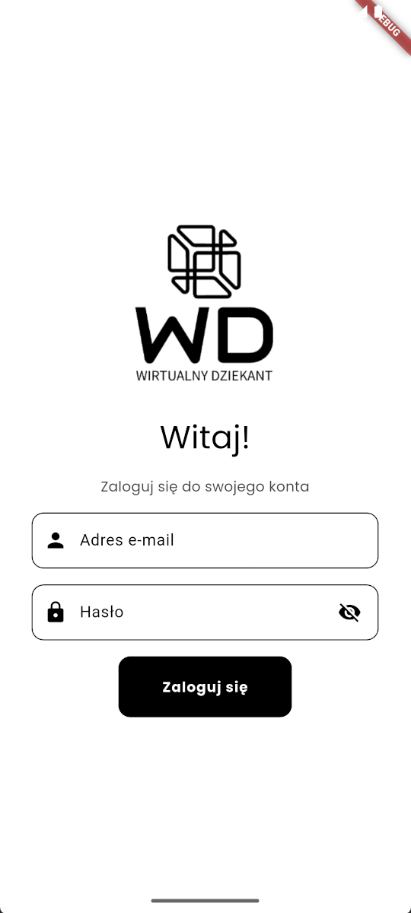
\includegraphics[width=0.5\textwidth]{rys/ekranlogowania.png}
	\caption{Ekran logowania}
	\label{rys:ekranlogowania2}
\end{figure}

\subsection{Ekran główny}

Po zalogowaniu użytkownik zostanie przekierowany na ekran główny. Na ekranie głównym znajduje się plan zajęć, który pokazuje nadchodzące zajęcia. Kliknięcie na konkretny dzień wyświetli szczegóły, takie jak sala, wykładowca i godziny. \textbf{Rys. \ref{rys:ekranglowny2} (s. \pageref{rys:ekranglowny2})}
\begin{figure}[h!]
	\centering
	
\includegraphics[width=0.5\textwidth]{rys/ekranplanzajec.png}
	\caption{Ekran główny}
	\label{rys:ekranglowny2}
\end{figure}


\newpage
\subsection{Przedmioty}
Aby zobaczyć jakie przedmioty mamy na danym semetrze należy kliknąć na ikonę Przedmioty. Na ekranie przedmioty znajduję się lista przedmitów jakie posiadamy w aktualnym semestrze, średnia ocen , oraz data zbliżających się egzaminów. \textbf{Rys. \ref{rys:Przedmiotyv3} (s. \pageref{rys:Przedmiotyv3})}
\begin{figure}[h!]
	\centering
	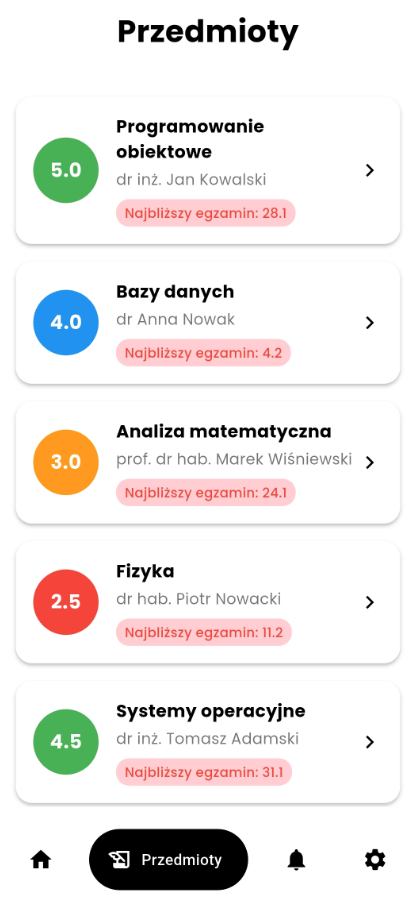
\includegraphics[width=0.55\textwidth]{rys/Przedmiotyv3.png}
	\caption{Ekran Przedmioty}
	\label{rys:Przedmiotyv3}
\end{figure}
\newpage
Jeżeli chcemy zobaczyć szczegóły danego przedmiotu (Np. wszystkie oceny). Nalęży kliknąć na szczałkę obok tego przedmiotu co poskutkuje przeniesieniem nas do jego szczegółów. \textbf{Rys. \ref{rys:Przedmiotyv4} (s. \pageref{rys:Przedmiotyv4})}
\begin{figure}[h!]
	\centering
	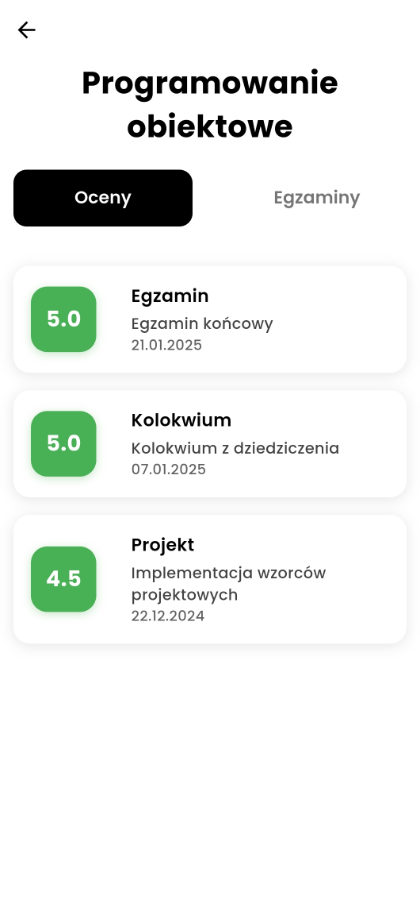
\includegraphics[width=0.55\textwidth]{rys/przedmiotyv4.png}
	\caption{Ekran szczegółowy dla danego Przedmiotu - Oceny}
	\label{rys:Przedmiotyv4}
\end{figure}
\newpage
Jeżeli chcielibyśmy przejść do szczegółów dotyczących Egzaminu dla danego przedmiotu należy kliknąć na okienko Egzaminy.  \textbf{Rys. \ref{rys:Przedmiotyv5} (s. \pageref{rys:Przedmiotyv5})}
\begin{figure}[h!]
	\centering
	
\includegraphics[width=0.55\textwidth]{rys/przedmiotyv5.png}
	\caption{Ekran szczegółowy dla danego Przedmiotu - Egzaminy}
	\label{rys:Przedmiotyv5}
\end{figure}

\newpage
\subsection{Ogłoszenia}

Aby zobaczyć ogłoszenia, należy kliknąć na ikonę Ogłoszenia w dolnym pasku nawigacyjnym. Po zrobieniu tego wyświetli się lista ogłoszeń. W zależności od ustawionego piorytetu danego ogłoszenia kolor boxa obok niego  będzię inny (Np. Pilne - Czerwony, Zwykłe - Szare). \textbf{Rys. \ref{rys:ekranpowiadomien} (s. \pageref{rys:ekranpowiadomien})}
\begin{figure}[h!]
	\centering
	
\includegraphics[width=0.5\textwidth]{rys/ekranpowiadomien.png}
	\caption{Ekran ogłoszeń}
	\label{rys:ekranpowiadomien}
\end{figure}
\newpage
Aby zobaczyć szczegóły danego ogłoszenie musimy je kliknąć. \textbf{Rys. \ref{rys:ogloszenieszcz} (s. \pageref{rys:ogloszenieszcz})}
\begin{figure}[h!]
	\centering
	
\includegraphics[width=0.55\textwidth]{rys/ogloszenieszcz.png}
	\caption{Szczegóły danego ogłoszenia}
	\label{rys:ogloszenieszcz}
\end{figure}
\newpage
Jeżeli na telefonie przyjdzie do nas powiadomie \textbf{Rys. \ref{rys:pushnot} (s. \pageref{rys:pushnot})}. To po kliknięciu na nie zostatniemy odrazu przekierowani do ekranu z ogłoszeniami \textbf{Rys. \ref{rys:pushnotv2} (s. \pageref{rys:pushnotv2})}.
\begin{figure}[h!]
	\centering
	
\includegraphics[width=0.7\textwidth]{rys/pushnot.png}
	\caption{Push notification}
	\label{rys:pushnot}
\end{figure}
\newpage
\begin{figure}[h!]
	\centering
	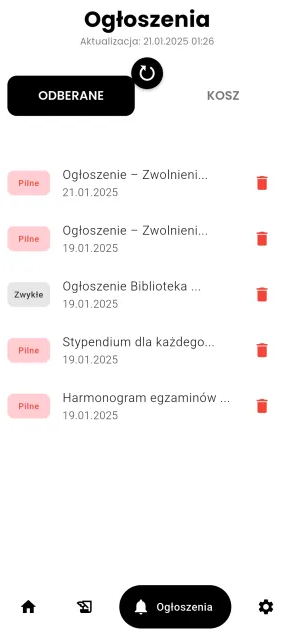
\includegraphics[width=0.6\textwidth]{rys/pushnotv2.png}
	\caption{Push notification}
	\label{rys:pushnotv2}
\end{figure}
\newpage

\subsection{Tryb offline - dostęp do zapisanych danych bez dostępu do Internetu}
\begin{figure}[htp!]
	\centering
	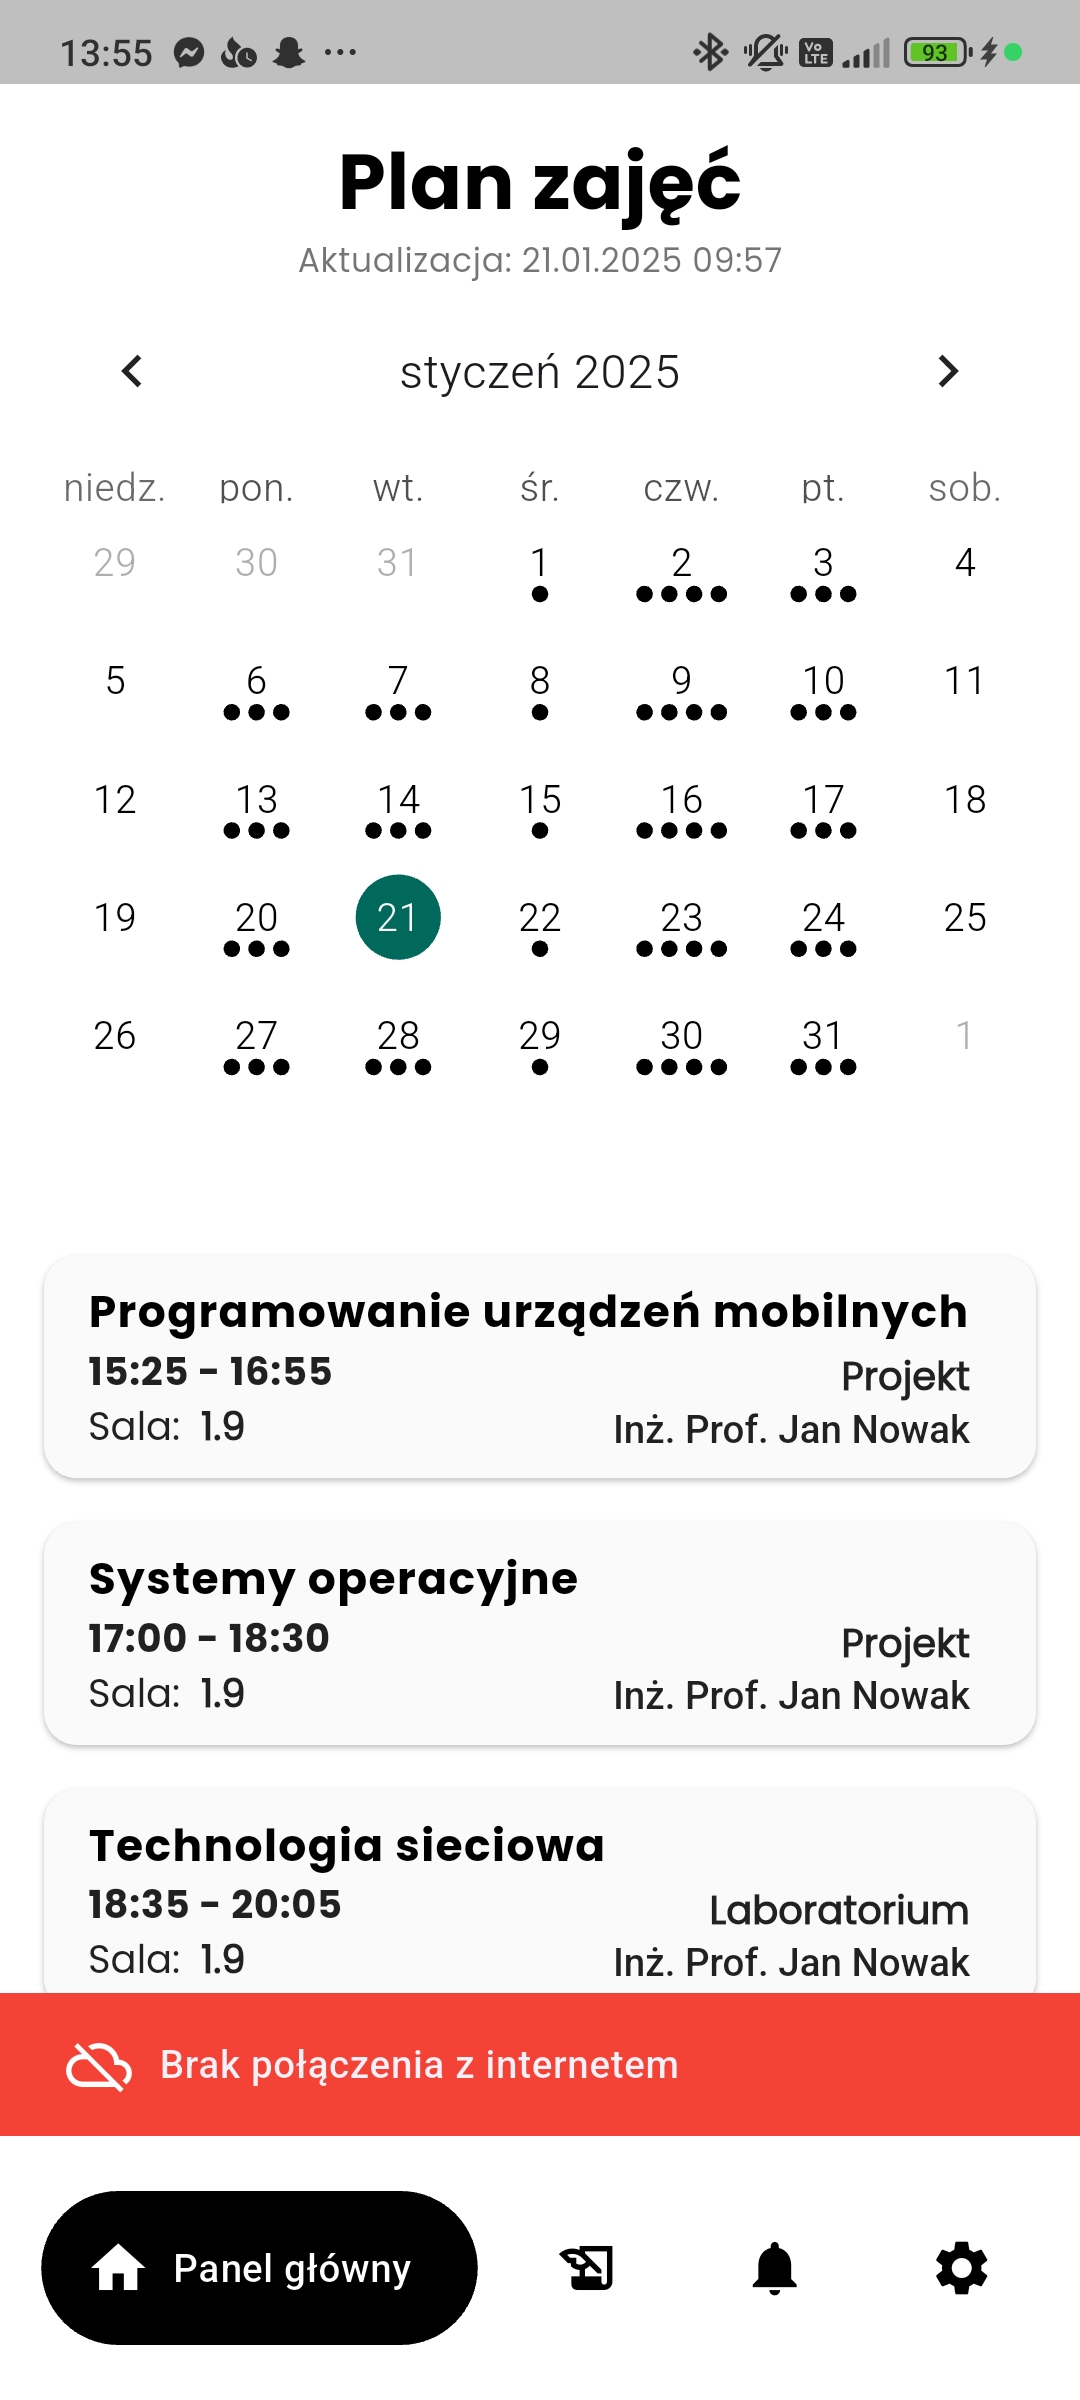
\includegraphics[width=0.6\textwidth]{rys/app_disconnected.jpg}
	\caption{Utracono połączenie z Internetem}
	\label{rys:pushnotv2}
\end{figure}
\newpage

\begin{figure}[htp!]
	\centering
	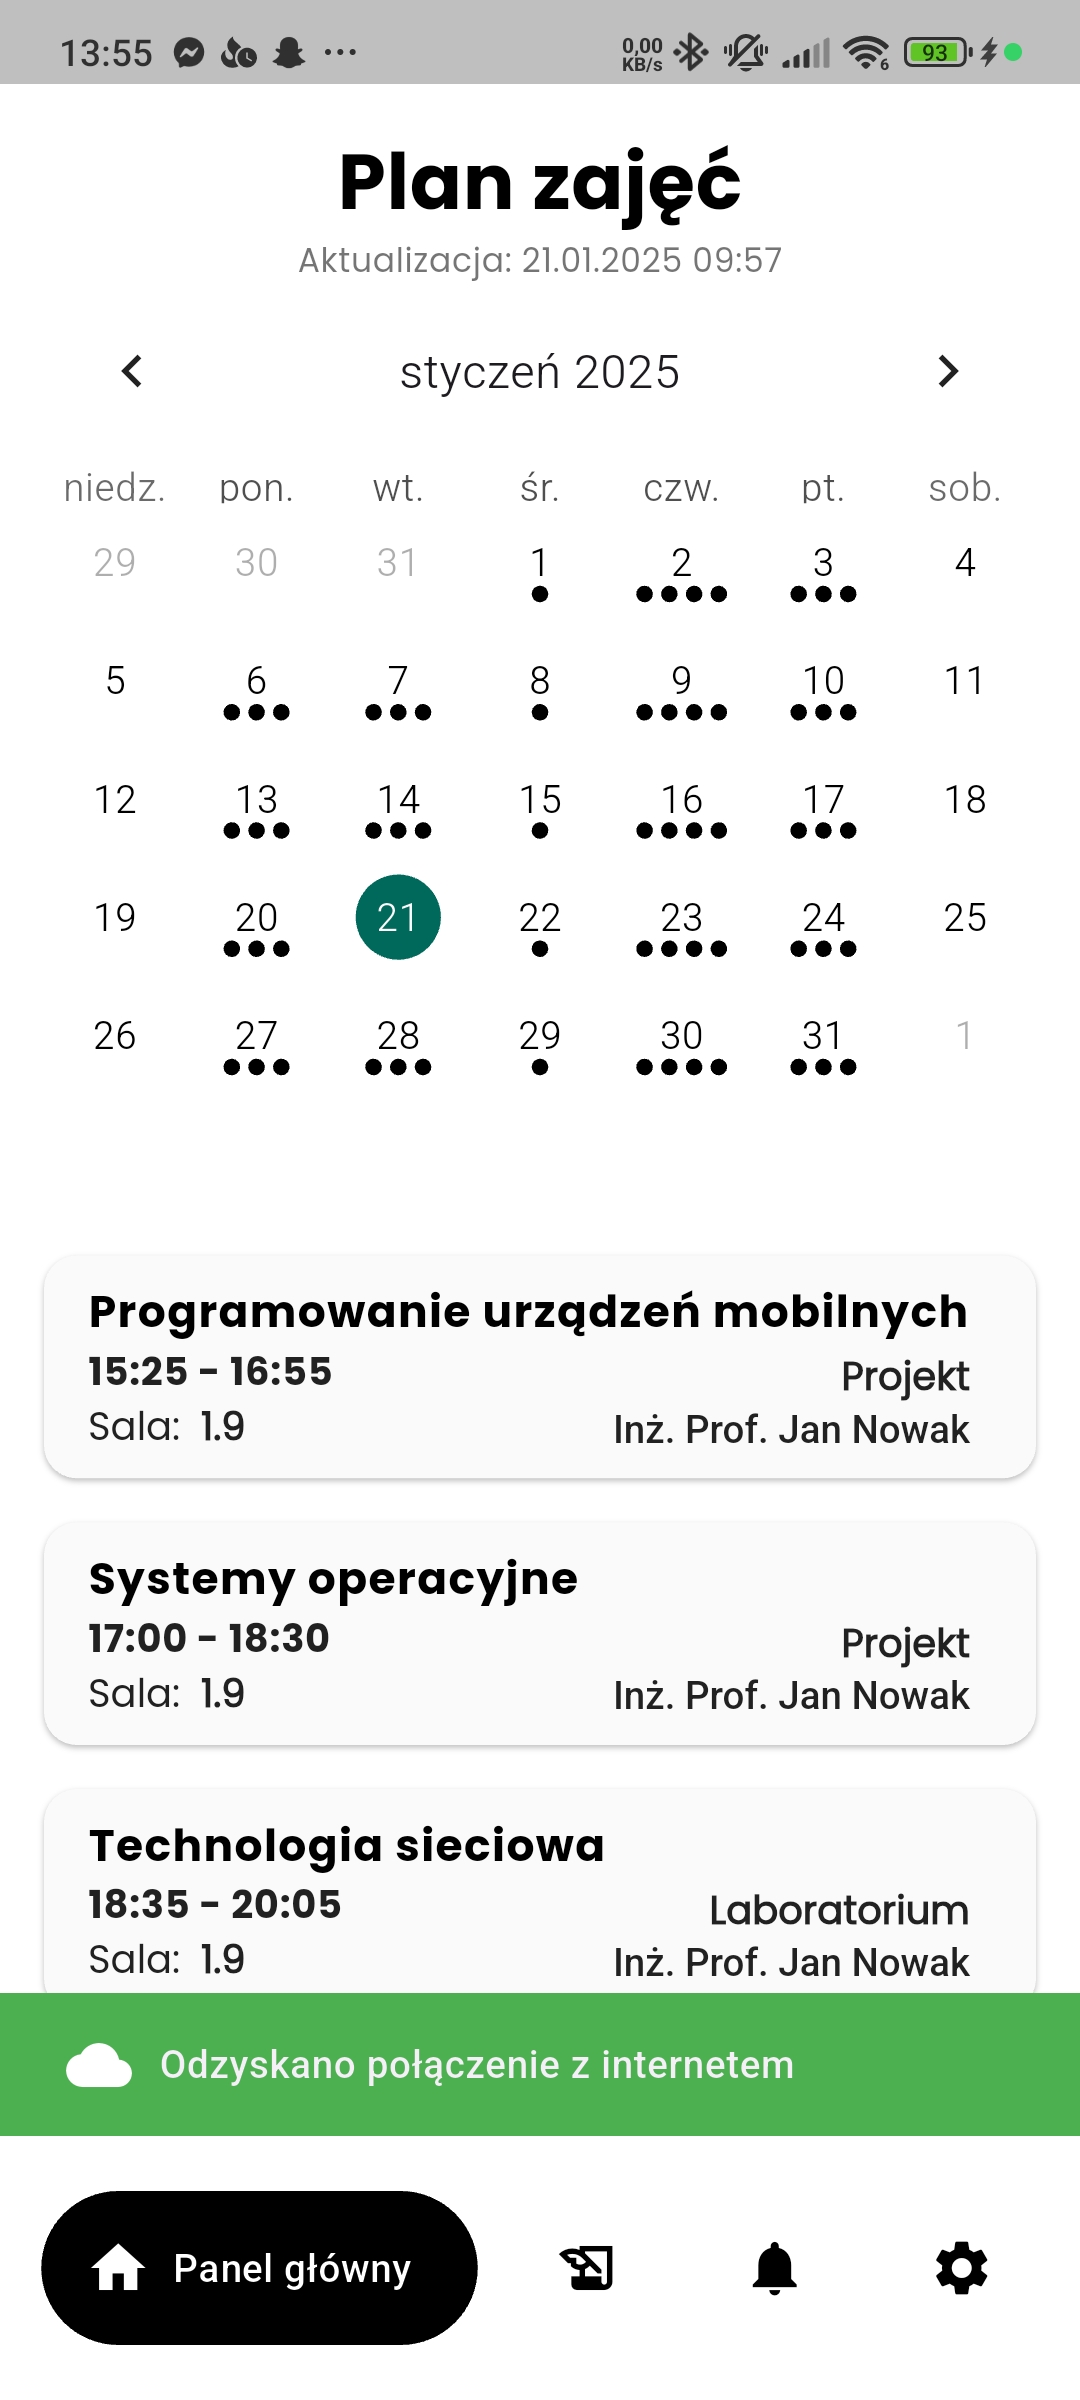
\includegraphics[width=0.6\textwidth]{rys/app_reconnected.jpg}
	\caption{Odzyskano połączenie z Internetem}
	\label{rys:pushnotv2}
\end{figure}

\newpage

\subsection{Ustawienia}

Aby przejść do ustawień, należy kliknąć na ikonę ustawień w dolnym pasku nawigacyjnym. W ustawieniach użytkownik może: \textbf{Rys. \ref{rys:ekranustawien1} (s. \pageref{rys:ekranustawien1})}

\begin{itemize}
	\item Włączyć lub wyłączyć tryb ciemny
	\item Zarządzać powiadomieniami
	\item Włączyć lub wyłączyć biometrię
\end{itemize}
\begin{figure}[htb!]
	\centering
	
\includegraphics[width=0.5\textwidth]{rys/ekranustawien.png}
	\caption{Ekran ustawień}
	\label{rys:ekranustawien1}
\end{figure}
\newpage
\subsubsection{Tryb ciemny}

Aby włączyć tryb ciemny, należy przełączyć odpowiedni przełącznik w ustawieniach. Aplikacja automatycznie zmieni motyw na ciemny. \textbf{Rys. \ref{rys:darkmode} ,\ref{rys:whitemode}(s. \pageref{rys:darkmode} , \pageref{rys:whitemode})}
\\\textbf{DarkMode ON}:
\begin{figure}[h!]
	\centering
	
\includegraphics[width=0.55\textwidth]{rys/darkmode.png}
	\caption{Włączenie darkmoda}
	\label{rys:darkmode}
\end{figure}
\newpage
\textbf{DarkMode OFF}:
\begin{figure}[h!]
	\centering
	
\includegraphics[width=0.55\textwidth]{rys/whitemode.png}
	\caption{Wyłączenie darkmoda}
	\label{rys:whitemode}
\end{figure}

\newpage
\subsubsection{Zarządzanie powiadomieniami}
W ustawieniach można włączyć lub wyłączyć powiadomienia dla różnych typów zdarzeń, takich jak nadchodzące zajęcia czy nowe oceny.\textbf{Rys. \ref{rys:notificationON}, \ref{rys:notificationOFF} (s. \pageref{rys:notificationON}, \pageref{rys:notificationOFF})}
\\\textbf{Powiadomienia ON:}
\begin{figure}[h!]
	\centering
	
\includegraphics[width=0.55\textwidth]{rys/biometricssONN.png}
	\caption{Zarządzanie powiadomieniami ON}
	\label{rys:notificationON}
\end{figure}
\newpage
\textbf{Powiadomienia OFF:}
\begin{figure}[h!]
	\centering
	
\includegraphics[width=0.55\textwidth]{rys/app_notifications_off.jpg}
	\caption{Zarządzanie powiadomieniami OFF}
	\label{rys:notificationOFF}
\end{figure}

\newpage
\subsubsection{Profil użytkownika}

Kliknięcie na avatar w ustawieniach przenosi użytkownika do ekranu profilu \textbf{Rys. \ref{rys:ekranustawien2} (s. \pageref{rys:ekranustawien2})}:, gdzie można
\begin{itemize}
	\item Zmienić zdjęcie profilowe
	\item Zobaczyć informacje o sobie, takie jak imię, nazwisko, adres e-mail
\end{itemize}
\begin{figure}[h!]
	\centering
	
\includegraphics[width=0.5\textwidth]{rys/ekranustawienv2.png}
	\caption{Ekran ustawień}
	\label{rys:ekranustawien2}
\end{figure}
\newpage
Aby zaktualizować zdjęcie należy kliknąć na przycisk \textbf{`Zaktualizuj Zdjęcie`}.Po kliknięciu mamy do wyboru 2 opcje (Wybierz z galerii, Zrób zdjęcie) \textbf{Rys. \ref{rys:ekranustawienv3} (s. \pageref{rys:ekranustawienv3})}
\begin{figure}[h!]
	\centering
	
\includegraphics[width=0.55\textwidth]{rys/ekranustawienv3.png}
	\caption{Wybór aktualizacji zdjęcia}
	\label{rys:ekranustawienv3}
\end{figure}
\newpage
Po zrobieniu zdjęcia Gdy wyszstko przebiegło pomyślnie powienien wyświetlić się zielony komunikat "Zdjęcie zostało zaktualizowane" co oznacza że zostało pomyślnie zaktualizowane w naszej bazy danych.  \textbf{Rys. \ref{rys:ekranustawienv4} (s. \pageref{rys:ekranustawienv4})}
\begin{figure}[h!]
	\centering
	
\includegraphics[width=0.55\textwidth]{rys/ekranustawienv4.png}
	\caption{Zdjęcie zostało poprawnie zrobione i do naszej bazy dancyh}
	\label{rys:ekranustawienv4}
\end{figure}
\newpage
\subsubsection{Biometria}
Po restracie apliakcji biometria pozwala na automatyczne logowanie się wcześniejszymi danymi poprzez odcisk palca przez co nie musimy na nowo wpisywać naszych danych.
\\Biomteria OFF \textbf{Rys. \ref{rys:biomteriaOFF} (s. \pageref{rys:biomteriaOFF})}:
\begin{figure}[h!]
	\centering
	
\includegraphics[width=0.55\textwidth]{rys/biometrics_off.png}
	\caption{Biomteria OFF}
	\label{rys:biomteriaOFF}
\end{figure}
\newpage
Biomteria ON \textbf{Rys. \ref{rys:biomteriaON} (s. \pageref{rys:biomteriaON})}:
\begin{figure}[h!]
	\centering
	
\includegraphics[width=0.55\textwidth]{rys/biometricssONN.png}
	\caption{Biometria ON}
	\label{rys:biomteriaON}
\end{figure}

\newpage
Gdy mamy włączoną biomterię to po wyłączeniu i właczeniu na nowo apikacji ta poprosi nas o podanie odcisku palca. Należy przyłożyć palec. Gdy weryfikacje się powiedzie to przeniesie nas do wnętrza aplikacji \textbf{Rys. \ref{rys:biomteriaON2} (s. \pageref{rys:biomteriaON2})}:
\begin{figure}[h!]
	\centering
	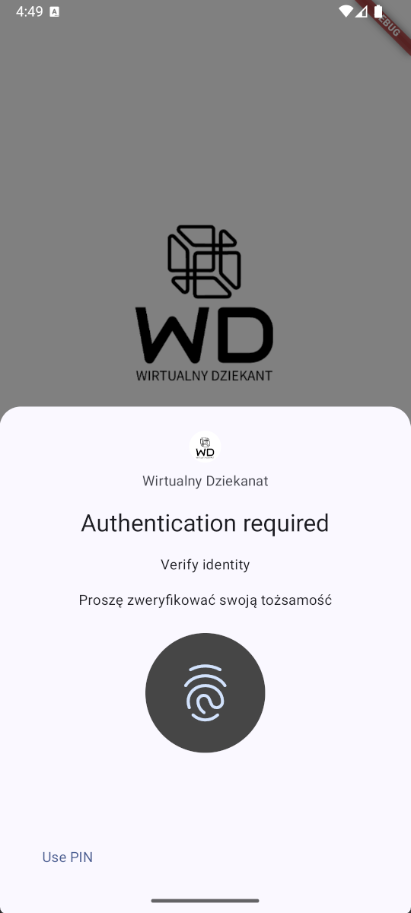
\includegraphics[width=0.55\textwidth]{rys/biometericON2.png}
	\caption{Poproszenie użytkownika o podanie odcisku palca}
	\label{rys:biomteriaON2}
\end{figure}

\newpage
\subsubsection{Wylogowanie}

Aby się wylogować, należy kliknąć na przycisk "Wyloguj się" na ekranie profilu. Użytkownik zostanie wylogowany i przekierowany na ekran logowania. \textbf{Rys. \ref{rys:wylogowanie} (s. \pageref{rys:wylogowanie})}

\begin{figure}[h!]
	\centering
	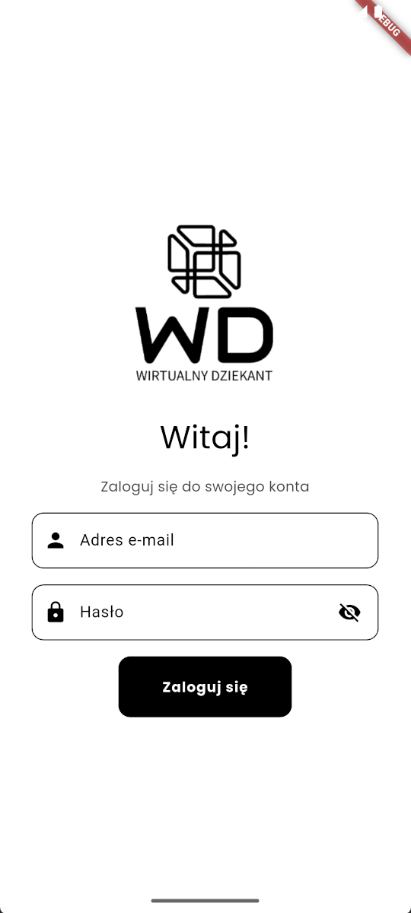
\includegraphics[width=0.6\textwidth]{rys/ekranlogowania.png}
	\caption{Widok po wylogowaniu}
	\label{rys:wylogowanie}
\end{figure}
\newpage
\subsection{Pull to refresh}
Aby użyć funkcji \textbf{pull to refresh} np. w panelu głównym musimy zrobić ruch palcem z góry aplikacji do środka (Powinno się utworzyć takie małe koło). Gdy już mamy palec na środku należy go puścić przez co naszę dane się automatycznie odświeżą. \textbf{Rys. \ref{rys:pull} (s. \pageref{rys:pull})}

\begin{figure}[h!]
	\centering
	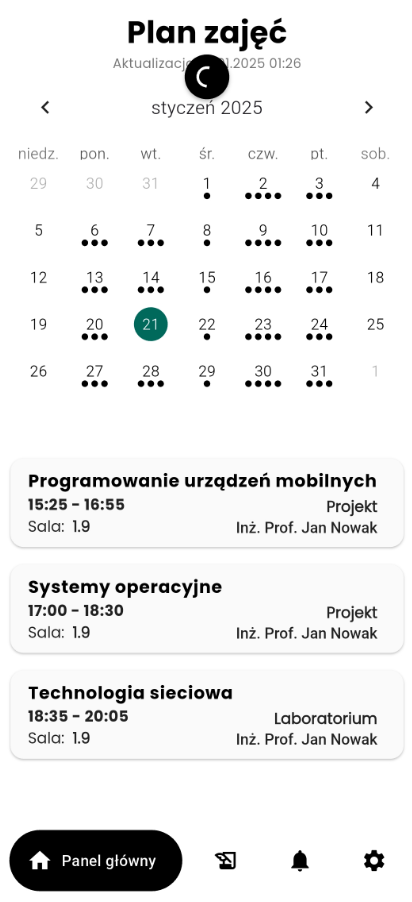
\includegraphics[width=0.55\textwidth]{rys/pull.png}
	\caption{Użycie pull to refresh}
	\label{rys:pull}
\end{figure}

\newpage
\subsection{Obsługa backendu}
Aby zalogować się do panelu administracyjnego backendu, należy przejść na stronę logowania i wprowadzić swoje dane uwierzytelniające. Po zalogowaniu użytkownik zostanie przekierowany do głównego interfejsu użytkownika, gdzie można zarządzać danymi aplikacji. \textbf{Rys. \ref{rys:be-login} (s. \pageref{rys:be-login})}

\begin{figure}[htp!]
	\centering
	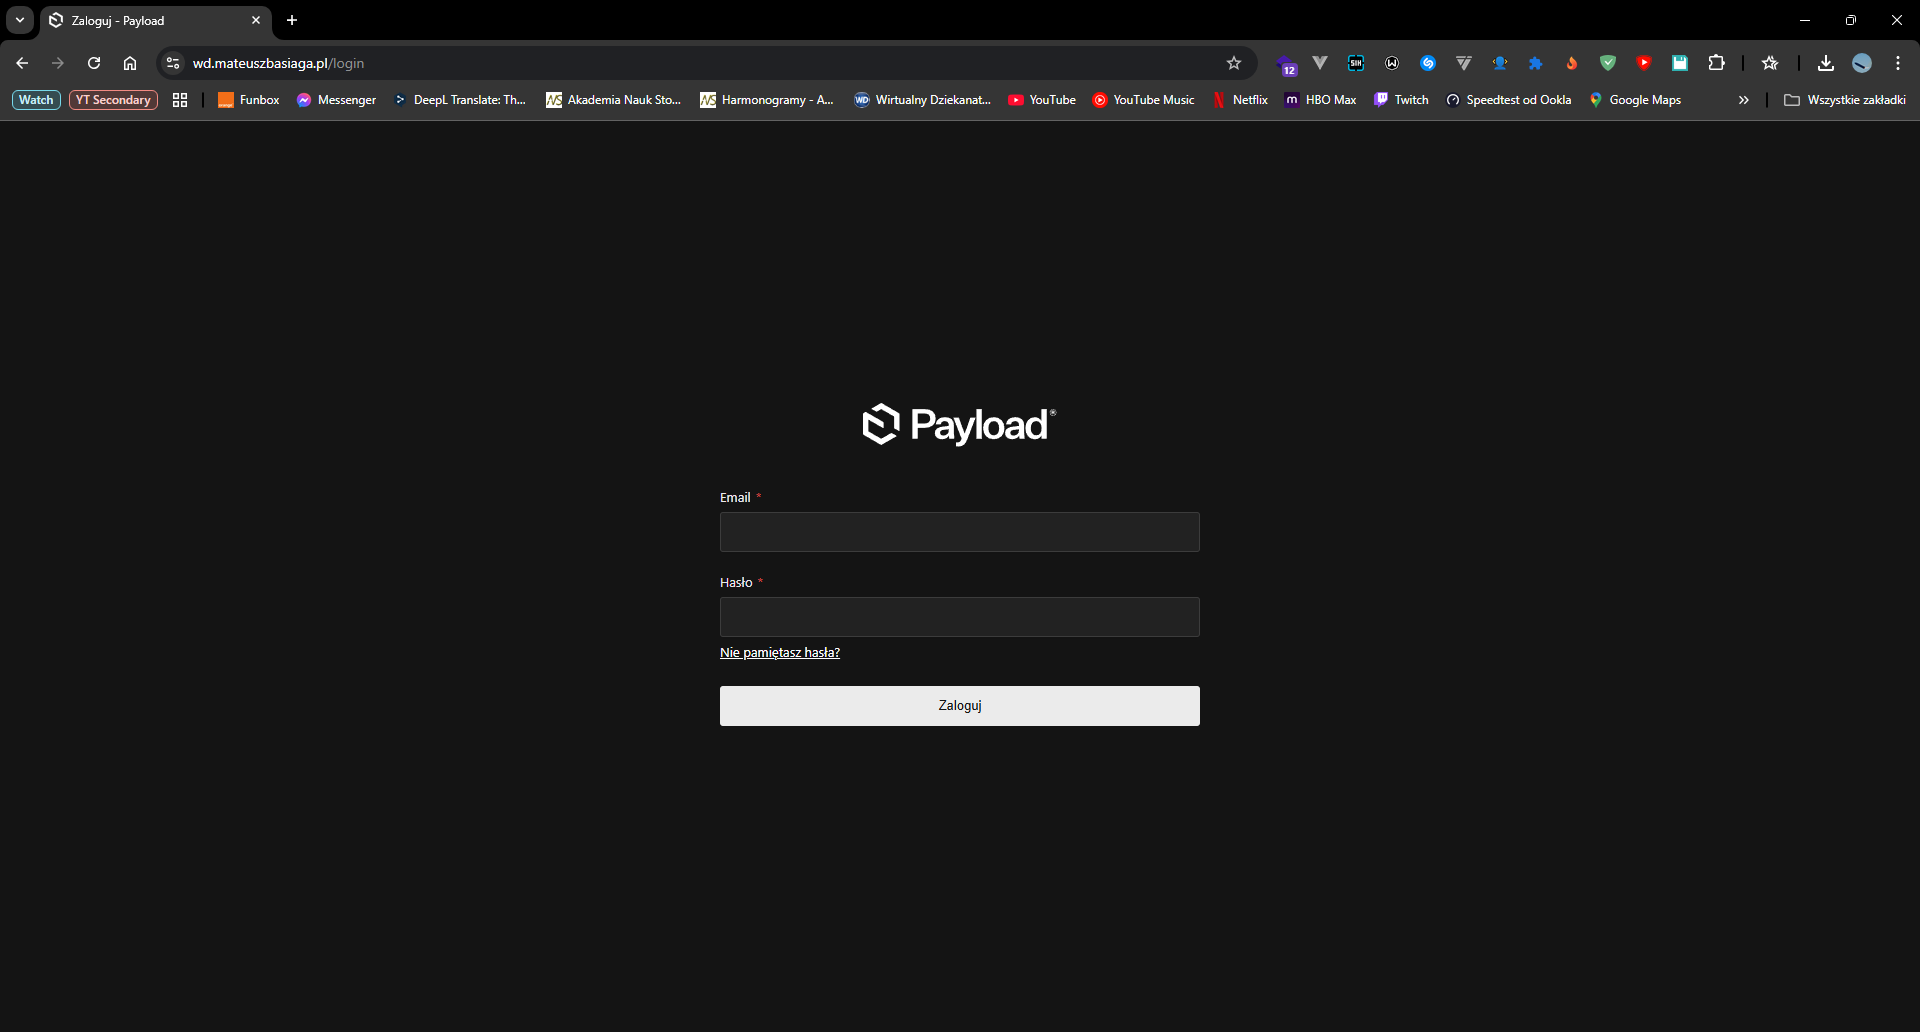
\includegraphics[width=\textwidth]{rys/be-login.png}
	\caption{Ekran logowania}
	\label{rys:be-login}
\end{figure}
\newpage
Główny interfejs użytkownika pozwala na przeglądanie i edytowanie danych, takich jak profile studentów, plan zajęć, ogłoszenia i inne. Użytkownik może również dodawać nowe wpisy oraz usuwać istniejące. \textbf{Rys. \ref{rys:be-main} (s. \pageref{rys:be-main})}

\begin{figure}[htp!]
	\centering
	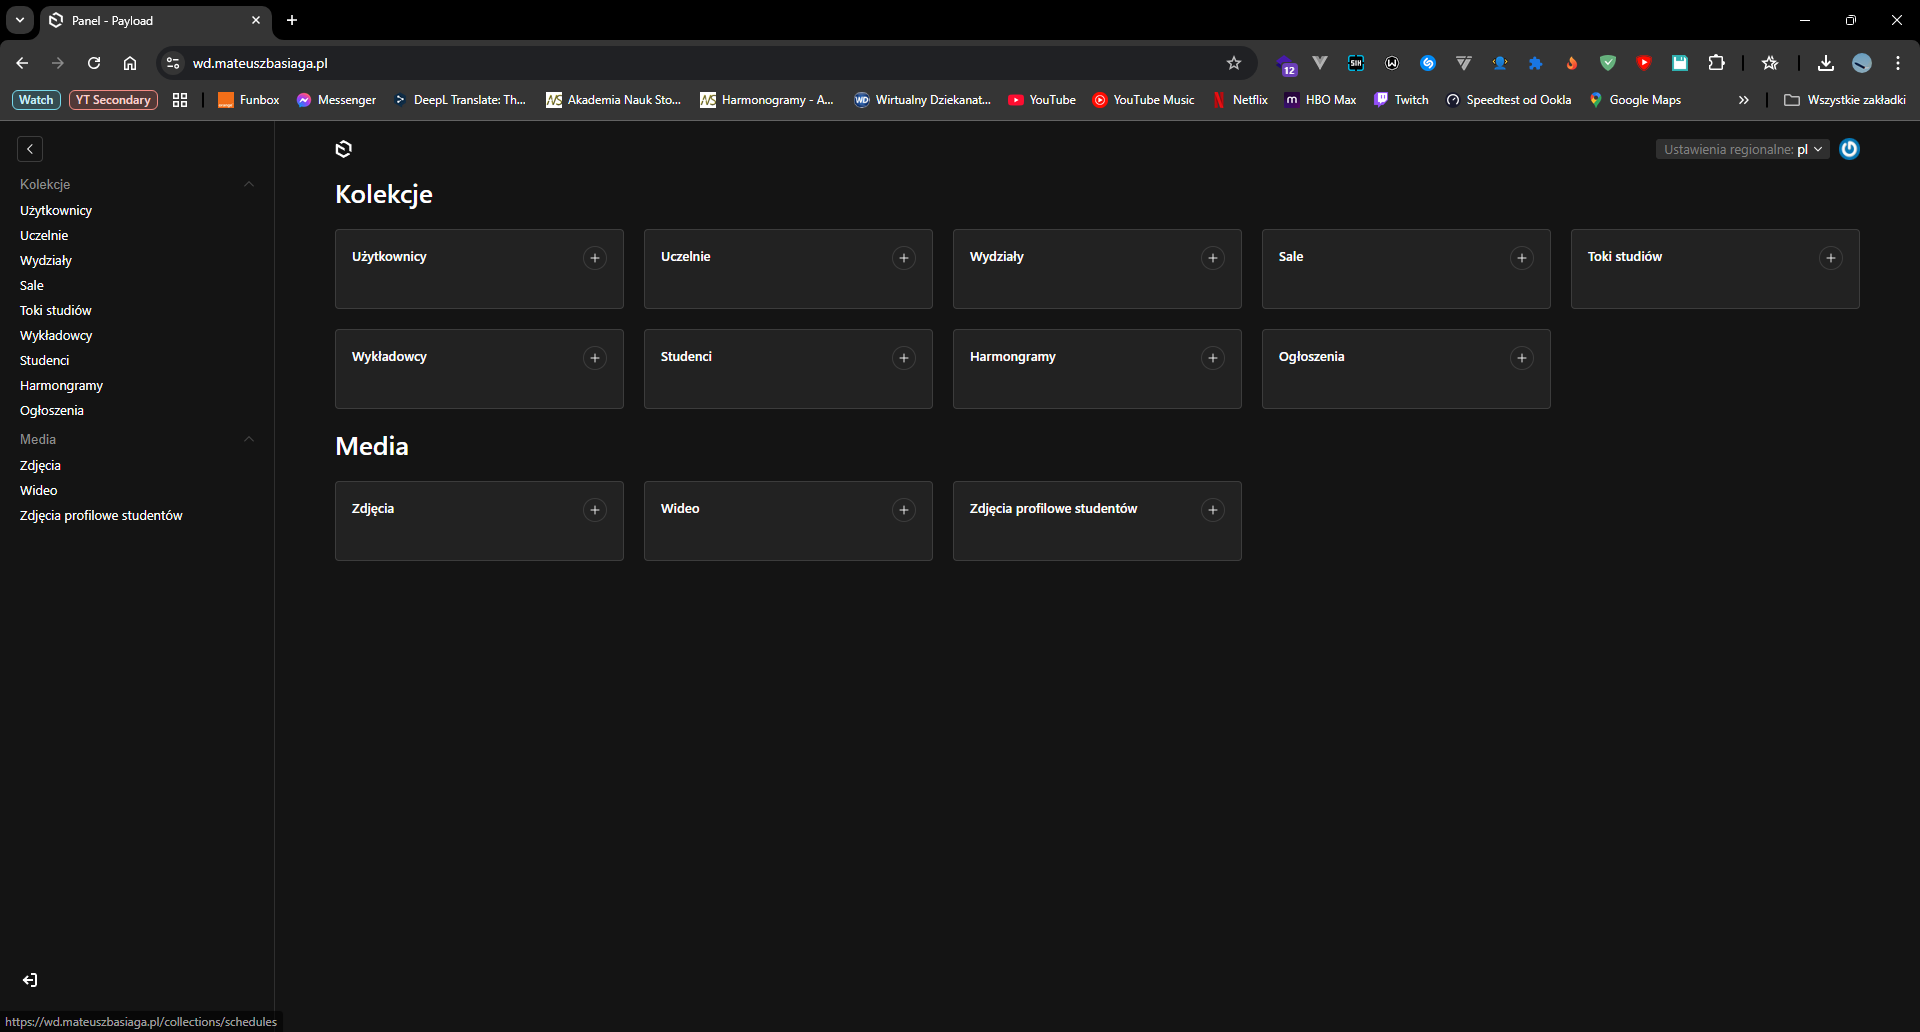
\includegraphics[width=\textwidth]{rys/be-main.png}
	\caption{Widok głównego interfejsu użytkownika}
	\label{rys:be-main}
\end{figure}

Profil studenta zawiera szczegółowe informacje o danym studencie, takie jak imię, nazwisko, adres e-mail, numer indeksu, rocznik, oceny i inne. Administrator może edytować te dane oraz dodawać nowe wpisy. \textbf{Rys. \ref{rys:be-student-profile} (s. \pageref{rys:be-student-profile})}

\begin{figure}[htp!]
	\centering
	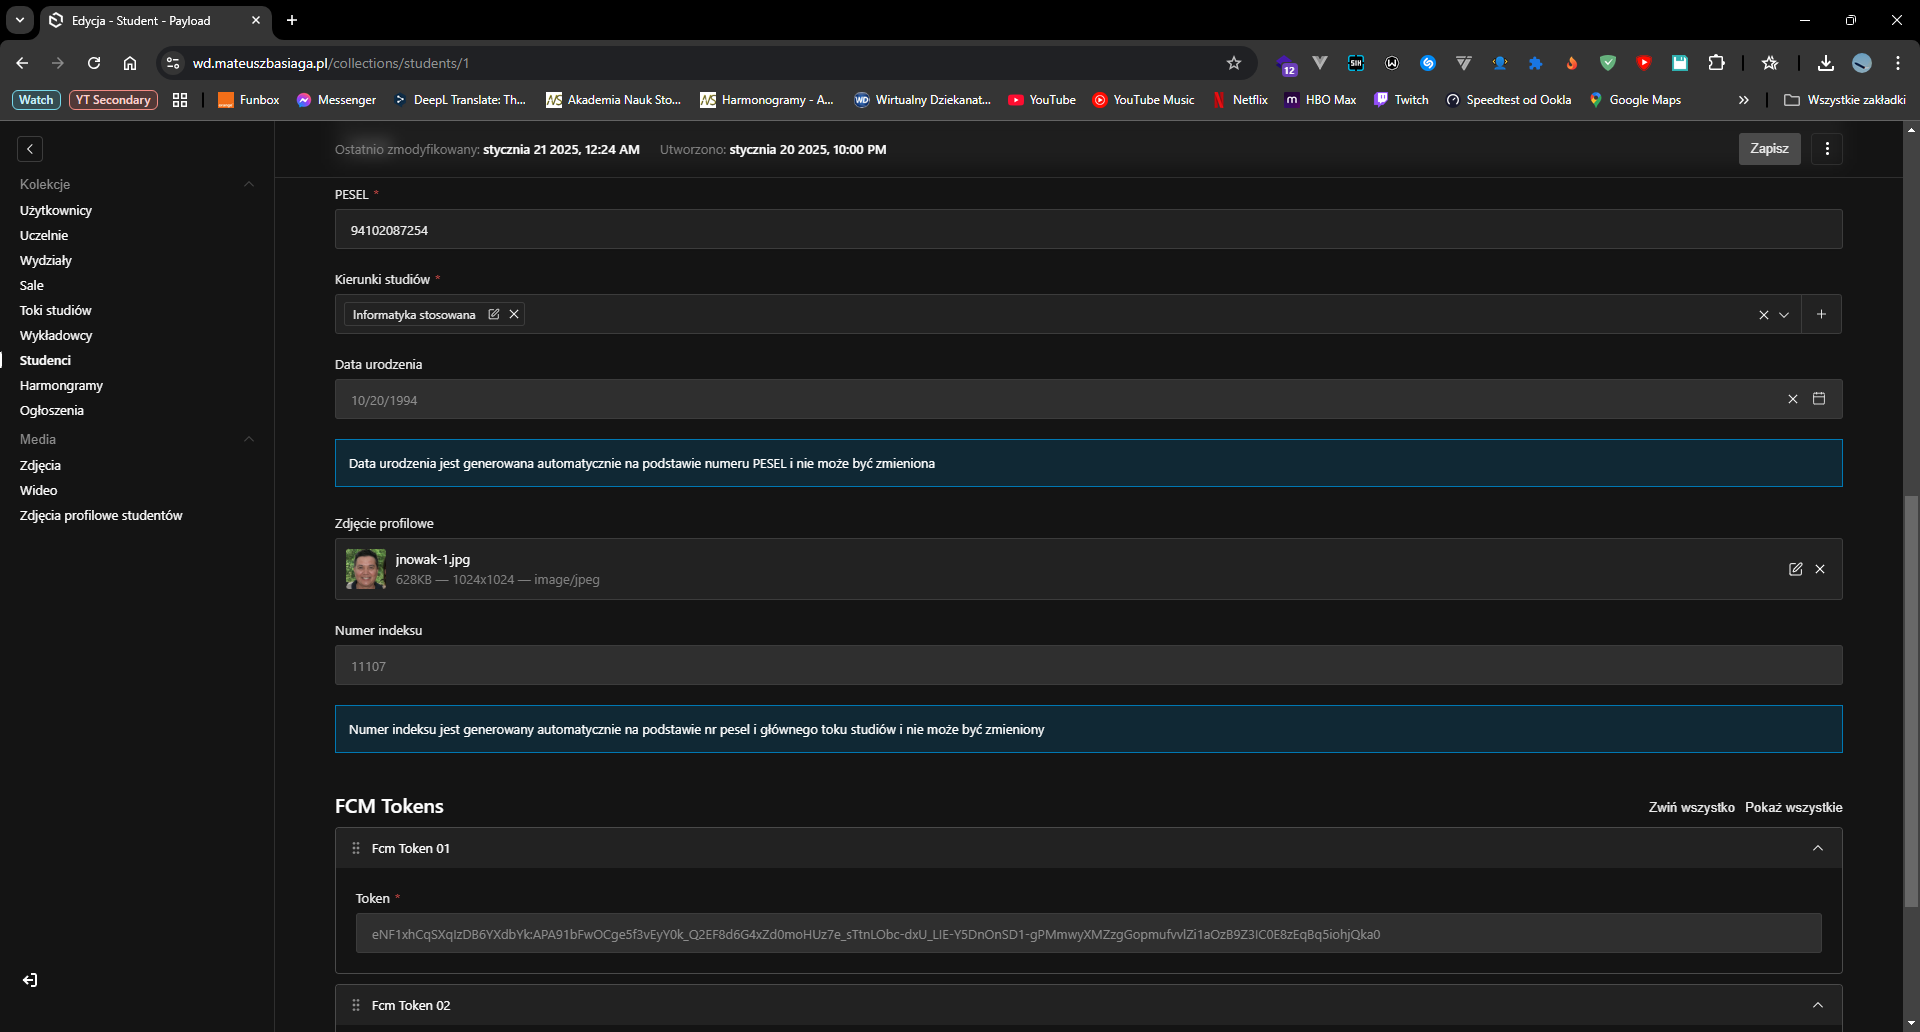
\includegraphics[width=\textwidth]{rys/be-student.png}
	\caption{Widok profilu studenta}
	\label{rys:be-student-profile}
\end{figure}
\newpage
Backend umożliwia również zarządzanie zdjęciami profilowymi studentów oraz innymi danymi multimedialnymi. Administrator może dodawać, edytować i usuwać zdjęcia profilowe. \textbf{Rys. \ref{rys:be-student-profi-pics} (s. \pageref{rys:be-student-profi-pics})}

\begin{figure}[htp!]
	\centering
	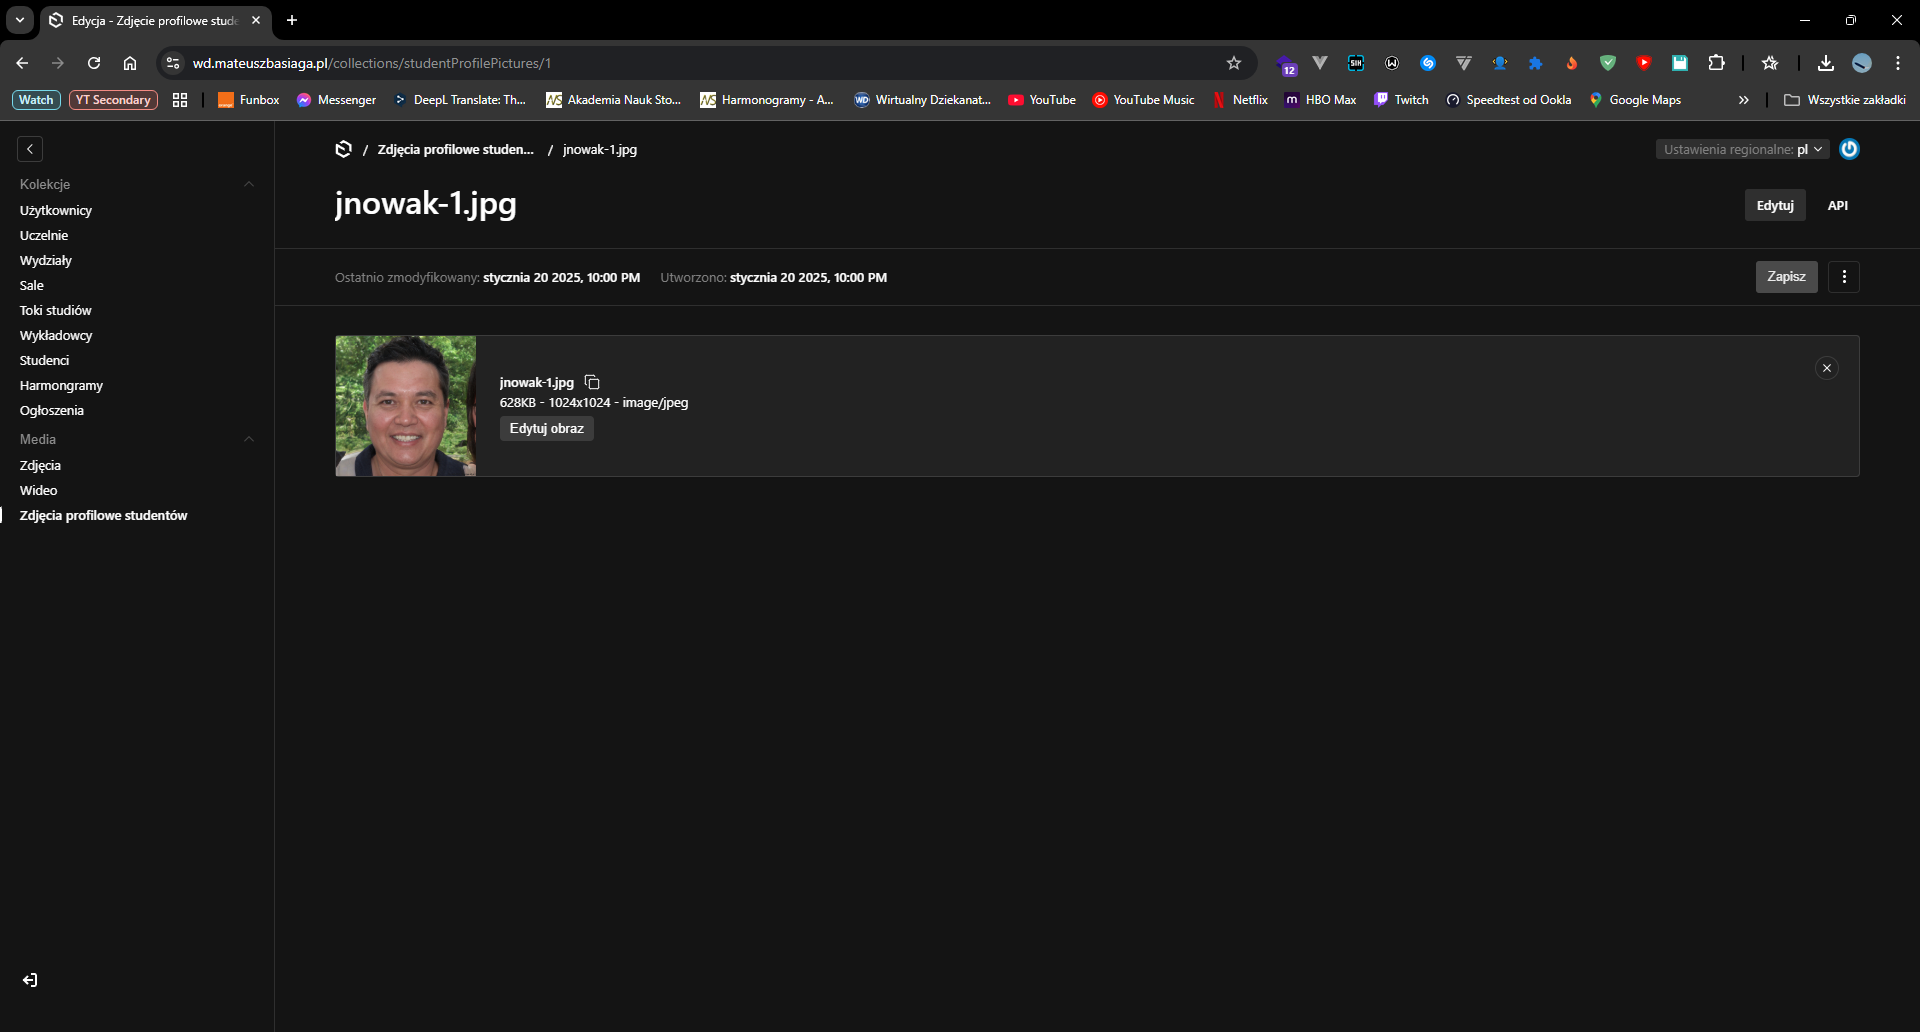
\includegraphics[width=\textwidth]{rys/be-student-prof-picture.png}
	\caption{Zdjęcia profilowe studentów - przykład danych multimedialnych}
	\label{rys:be-student-profi-pics}
\end{figure}

Plan zajęć można przeglądać i edytować za pomocą interfejsu backendu. Administrator może dodawać nowe zajęcia, edytować istniejące oraz usuwać wpisy. Plan zajęć jest synchronizowany z aplikacją mobilną, dzięki czemu studenci mają zawsze aktualne informacje. \textbf{Rys. \ref{rys:be-schedule} (s. \pageref{rys:be-schedule})}

\begin{figure}[htp!]
	\centering
	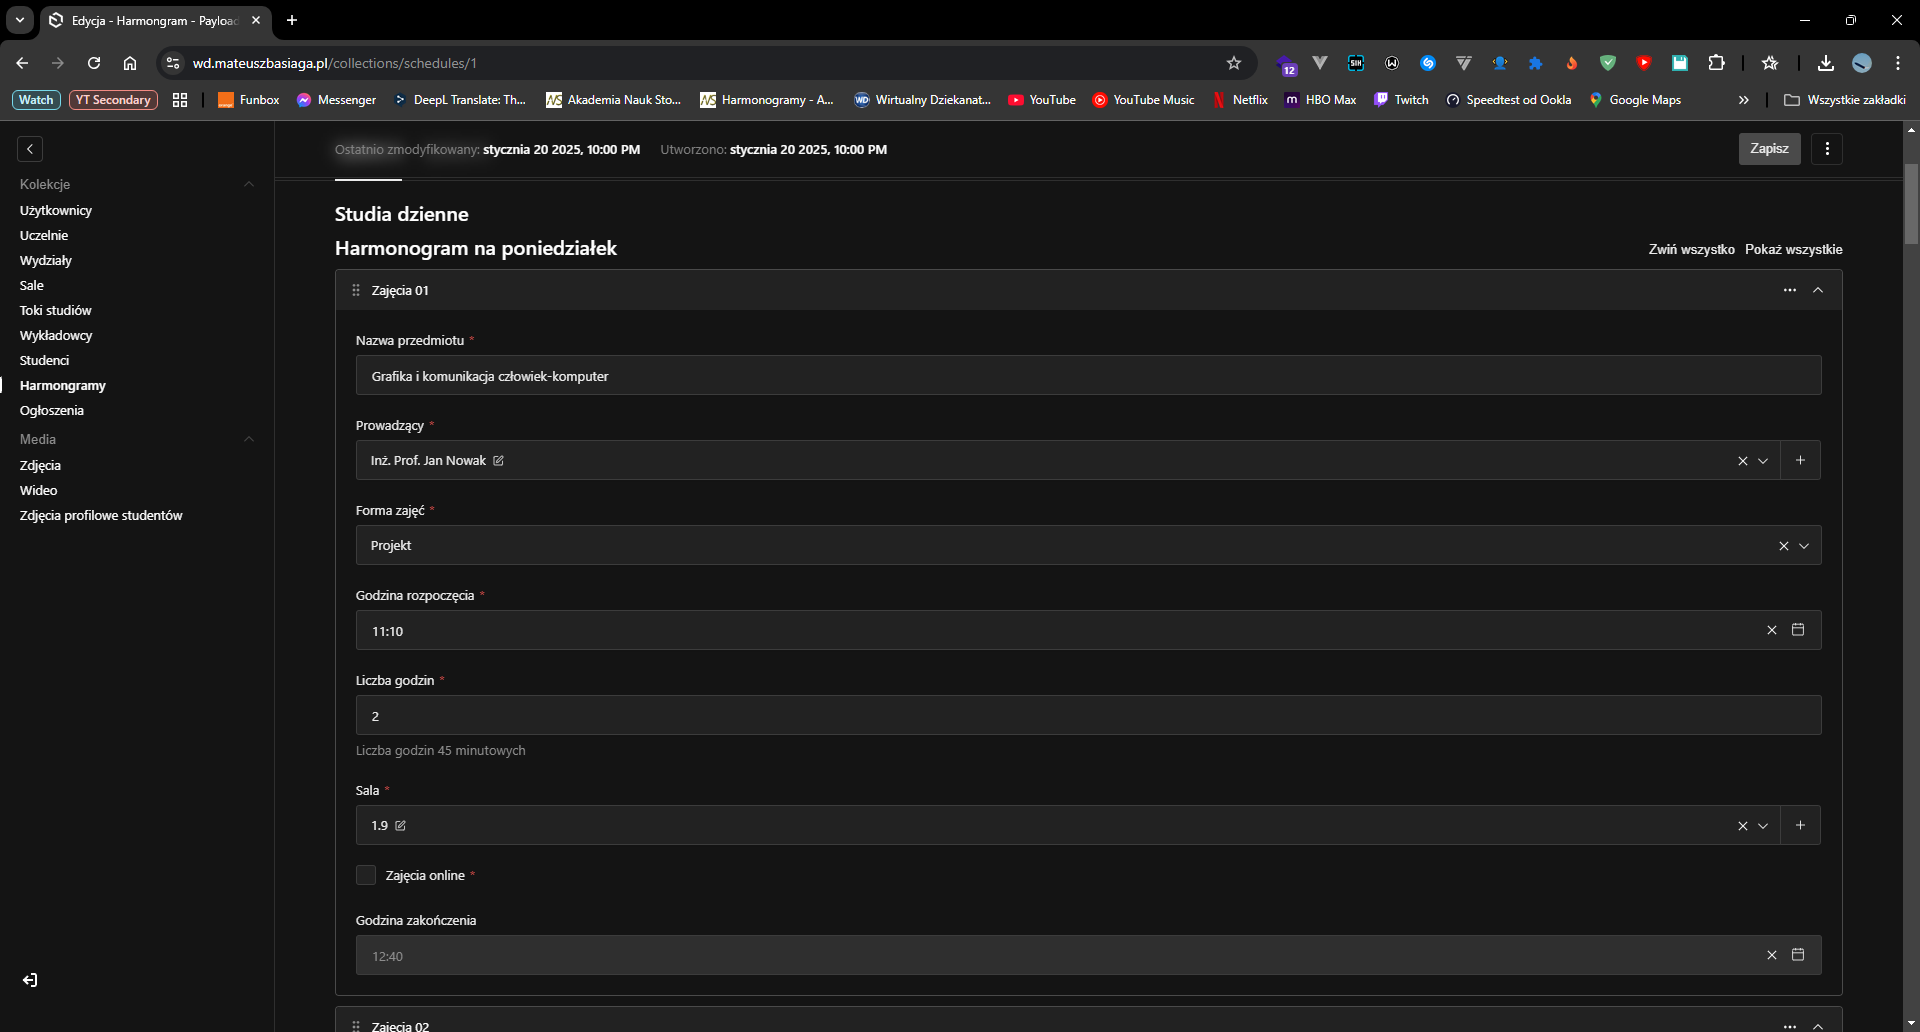
\includegraphics[width=\textwidth]{rys/be-schedule.png}
	\caption{Widok planu zajęć toku studiów}
	\label{rys:be-schedule}
\end{figure}
\newpage
Ogłoszenia można zarządzać za pomocą interfejsu backendu. Administrator może dodawać nowe ogłoszenia, edytować istniejące oraz usuwać wpisy. Ogłoszenia są synchronizowane z aplikacją mobilną, dzięki czemu studenci są na bieżąco informowani o ważnych wydarzeniach. \textbf{Rys. \ref{rys:be-announcement} (s. \pageref{rys:be-announcement})}

\begin{figure}[htp!]
	\centering
	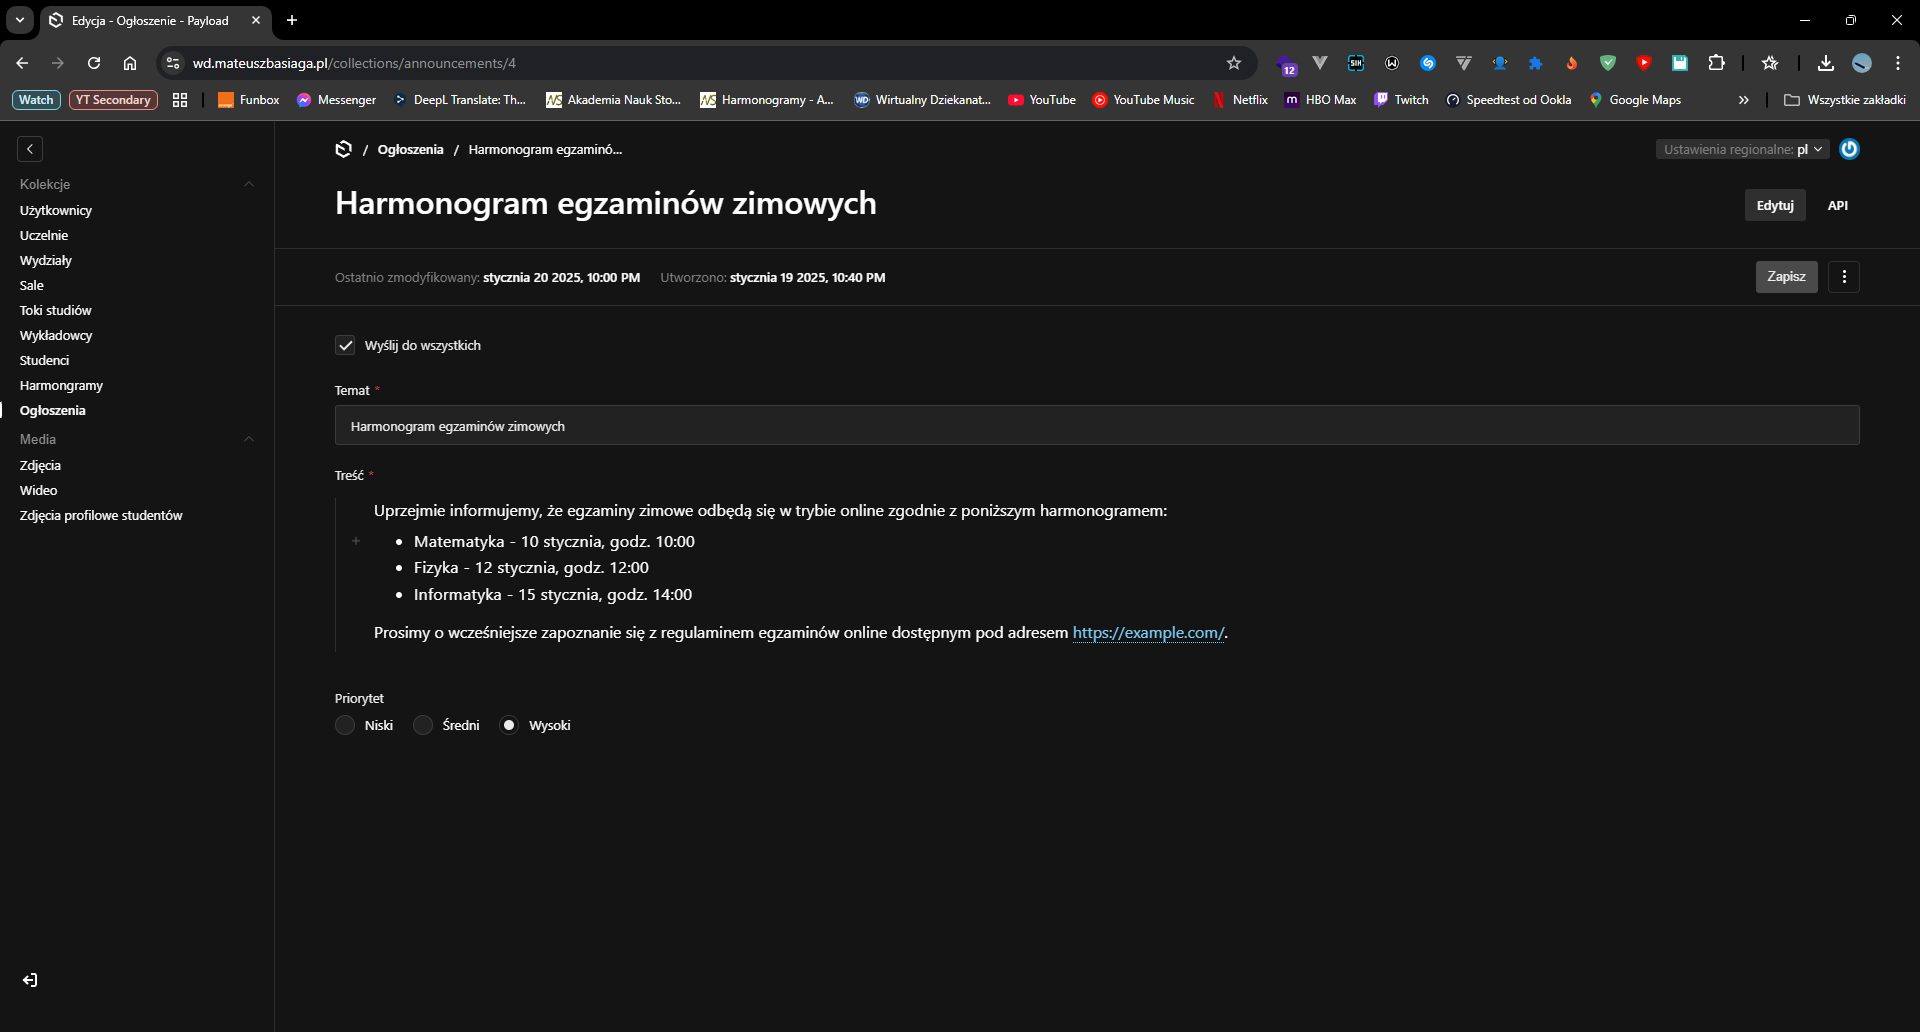
\includegraphics[width=\textwidth]{rys/be-announcement.png}
	\caption{Widok ogłoszenia}
	\label{rys:be-announcement}
\end{figure}

\nocite{www1}
\nocite{www2}
\nocite{www3}
\nocite{www4}
\nocite{www5}
\nocite{www6}
\nocite{www7}
\nocite{www8}
\nocite{www9}
\nocite{www10}
\nocite{www11}
\nocite{www12}


%%%%%%%%%%%%%%%%%%% koniec treść główna dokumentu %%%%%%%%%%%%%%%%%%%%%
\newpage
% \addcontentsline{toc}{section}{Literatura}
% Modified by: Maciej Wójs  
\printbibliography[heading=bibnumbered, label=Literatura, title=Literatura]

\newpage
\hypersetup{linkcolor=black}
\renewcommand{\cftparskip}{3pt}
\clearpage
\renewcommand{\cftloftitlefont}{\Large\bfseries\sffamily}
\listoffigures
\addcontentsline{toc}{section}{Spis rysunków}
\thispagestyle{fancy}

\newpage
\renewcommand{\cftlottitlefont}{\Large\bfseries\sffamily}
\def\listtablename{Spis tabel}
\addcontentsline{toc}{section}{Spis tabel}\listoftables
\thispagestyle{fancy}

\newpage
\renewcommand{\cftlottitlefont}{\Large\bfseries\sffamily}
\renewcommand\lstlistlistingname{Spis listingów}
\addcontentsline{toc}{section}{Spis listingów}\lstlistoflistings
\thispagestyle{fancy}

%lista rzeczy do zrobienia: wypisuje na koñcu dokumentu, patrz: pakiet todo.sty
\todos
%koniec listy rzeczy do zrobienia
\end{document}
